% gjilguid2e.tex
% V2.0 released 1998 December 18
% V2.1 released 2003 October 7 -- Gregor Hutton, updated the web address for the style files.

\documentclass{gji}
%\usepackage{timet}
\usepackage{amsmath}
\usepackage{graphicx}
%\usepackage{lineno}
%\linenumbers


\graphicspath{{./paper_figures/publishable/}}



\title[Comparisons of Love wave amplitude decay]
  {Comparisons of Love wave amplitude decay \\for colocated rotation and translation measurements}
\author[Bryant Chow]
  {Bryant Chow,$^1$\thanks{Now at Victoria University of Wellington, School of Geography, Environment and Earth Sciences, Cotton Building, Gate 7 Kelburn Parade, Wellington, New Zealand 6012} 
  Joachim Wassermann,$^1$
  Bernhard Schuberth,$^1$  \vspace{2mm}\\
  \LARGE{{\normalfont C\' eline Hadziiannou,$^{1,2}$ 
  Stefanie Donner$^{1,3}$ and
   Heiner Igel$^1$}}\vspace{2mm}  \\
  $^1$ Department of Earth and Environmental Sciences, Ludwig-Maximilians-University Munich, Theresienstra\ss e 41, D-80333 Munich, Germany.\\
  $^2$ Department of Earth Science, University of Hamburg, Bundesstra\ss e 55, D-20146 Hamburg, Germany\\
  $^3$ Federal Institute for Geosciences and Natural Resources, Stilleweg 2, D-30655 Hannover, Germany \\E-mail: bryant.chow@vuw.ac.nz
  }
\date{}
\pagerange{\pageref{firstpage}--\pageref{lastpage}}
\volume{}
\pubyear{}

%\def\LaTeX{L\kern-.36em\raise.3ex\hbox{{\small A}}\kern-.15em
%    T\kern-.1667em\lower.7ex\hbox{E}\kern-.125emX}
%\def\LATeX{L\kern-.36em\raise.3ex\hbox{{\Large A}}\kern-.15em
%    T\kern-.1667em\lower.7ex\hbox{E}\kern-.125emX}
% Authors with AMS fonts and mssymb.tex can comment out the following
% line to get the correct symbol for Geophysical Journal International.
\let\leqslant=\leq

\newtheorem{theorem}{Theorem}[section]

\begin{document}

\label{firstpage}

\maketitle

\begin{summary}
The broad-band surface wave magnitude equation assigns magnitude based on station-receiver distance and peak surface wave amplitude. It is standard practice to use the vertical component of peak ground velocity, so that only contributions from the vertical component of Rayleigh waves are present in the surface wave train. With the advent of rotational ground motion data from instruments such as ring laser gyroscopes and fiber-optic gyroscopes, it is possible to consistently measure peak amplitudes of rotations about three orthogonal axes for transient seismic waves. In the surface wave train, observations of vertical rotations are theoretically only sensitive to the transverse nature of Love waves, unaffected by either component of Rayleigh waves. We use this concept to study the amplitude decay of rotations verse translations, and determine the necessity of separate surface wave magnitude equations for Love and Rayleigh waves. Utilizing a large database of recorded seismic events of colocated translations and rotations, collected in Wettzell, Germany, we empirically define new magnitude scales for multiple measured observables: rotation rate, rotation, vertical velocity and transverse velocity. Results indicate that rotation amplitudes decay faster over distance compared to velocity amplitudes, and that the current surface wave magnitude equation is insufficient for predicting the amplitudes of either observable. Synthetic seismograms were produced using the spectral element method code Specfem3D Globe to compare against observations. Findings suggest that the current global models available for forward simulation are inadequate for accurately predicting amplitudes, and recreating the observed amplitude decay of both translations and rotations.
\end{summary}

\begin{keywords}
magnitude, rotational motions, amplitude decay, surface waves
\end{keywords}

\section{Introduction} 
% rotations are gaining traction, large catalog of events
For over a decade, the application of ring laser gyroscope technology to the field of seismology has allowed for near-continuous and direct measurements of rotational ground motions. An ever growing number of observations from seismic events of varying size, distance and source mechanism, has been collected in an expansive catalog of waveform recordings for both direct rotation, and colocated translation measurements.
%> we routinely compare amplitude ratios for phase velocities
Previous work on this unique waveform dataset includes phase comparisons of translations and rotations with estimations of horizontal phase velocities \cite{igel2005rotational},
automatic standardized processing of rotation and translation data \cite{salvermoser2017event}, and
variations of surface wave energy in oceanic microseisms \cite{tanimoto2016seasonal}.
Much of this preceding work however, focuses on single events, or collections of non-earthquake sources.

%> we want to understand how rotations decay compared to translations
%> how do we do this? we make 'magnitude scales' to quantify decay characterstics
%> these are not real magnitudes because we are geographically biased and we are not avera
%ging over hundreds of instruments like is common
In this paper, we aim to characterize and understand the differences in amplitude decay behavior of rotational and translational ground motion for a large number of seismic events. To do this, we make use of a sizeable catalog of earthquake data, as measured by an observatory based ring laser gyroscope, and colocated broadband translation sensor. By processing rotation and translation observations in a near identical manner, we hope to directly compare results over a large set of event magnitudes, epicentral distances and  azimuths. We additionally seek to use this information to better understand decay characteristics of Love and Rayleigh waves.

This paper builds on results previously shown by Igel et al. \shortcite{igel2007broad}, 
where the question was posed: whether observed peak rotation amplitudes matched with expected values given by the surface wave magnitude equation. 
% new
As a relatively new observable, rotational ground motion does not share the historical record of translations; there exist no empirical relationships such as magnitude equations, which are constantly referred to in literature and public outreach. As a result, we find it important to begin establishing these relationships for our new observable.
%new
At the time of Igel et al. \shortcite{igel2007broad}, a limited number of recorded events lead to a small sample size. With a larger number of events currently available, we attempt to readdress this question. We approach the problem by deriving our own magnitude scales, with which we can quantify the decay characteristics of rotations and translations. Since this instrumental setup is relatively unique, we are restricted to single station observations. In order to provide comparisons to our observations, global 3D synthetic simulations were run with the spectral element code Specfem 3D Globe \cite{komatitsch2002spectrala} \cite{komatitsch2002spectralb}. 

With these observations, we aim to make quantitative statements on surface wave amplitude decay, as well as to provide magnitude scale equations that may prove useful in determining expected rotation amplitudes from seismic events.

\subsection{Rotational Ground Motions}
To fully describe rigid body motion at a point, three components of translation, and three components of rotation must be defined \cite{stein2009introduction}. In seismology, standard practices make use of translation only, which means recorded motions only approximate the rigid body motion, and can potentially be polluted by rotational signals which cannot be separated from physical effects \cite{igel2005rotational}, \cite{aki2002quantitative}.  Rotational ground motions induced by seismic events can currently be observed through direct measurement, and through array analysis of translation sensors \cite{spudich1995transient}.
In the latter, spatial gradients are taken between instruments in adequately spaced array of translation sensors, in order to derive components of the strain tensor. Shortcomings of array based methods, however, include the necessity for multiple sensors and careful consideration for array spacing and geometry. With unique instrument designs, however, direct gradient measurements from a single instrument are possible \cite{schreiber2006ring}. %different rotation sensors

Observations for this study were recorded by the Gro\ss ring (G-ring) \cite{schreiber2006ring} \shortcite{schreiber2006geosensor}, a 4x4m helium-neon ring laser gyroscope, located at the Geodetic Fundamentalstation in Wettzell, Germany (49.144$^\circ$N, 12.87$^\circ$E). The G-ring operates on the principle of Sagnac interferometry \cite{stedman1997ring}, which relates interference of counter propagating light beams to absolute rotation rate, through the following equation, 

\begin{equation}\label{eq:sagnac}
	\delta f = \frac{4A}{\lambda P}\mathbf{n}\cdot \mathbf{\Omega},
\end{equation}

\noindent where the constants are given by instrument area A, perimeter P and operating light wavelength $\lambda$. Equation \ref{eq:sagnac} relates an observable beat frequency $\delta f$ [Hz] to absolute rotation rate $\Omega$ [rad/s].

It is important to note that given stable instrument geometry and lasing, changes to the beat frequency $\delta f$, can only be introduced by changes to the inner product of the plane normal {\bfseries n} with the rotation rate direction $\mathbf{\hat{\Omega}}$ (e.g. through instrumental tilt), and through externally induced rotations (e.g. the passing of seismic waves). It has been shown that changes to the inner product as produced by tilt are one to two orders of magnitude smaller than rotations produced by passing seismic waves \cite{mcleod1998comparison} \cite{schreiber2006ring} \shortcite{schreiber2006geosensor}, this provides the unique benefit that the G-ring (and other instruments operating on this principle) is theoretically insensitive to translations.

\subsubsection{Phase velocity relation}\label{phasevel}
It has been shown that for a simple plane wave, the amplitudes of vertical rotation rate $\Omega_z$  and transverse acceleration $\ddot{u}_t$ can be related through the equation 

\begin{equation}\label{eq:phasevelocity}
	\frac{\ddot{u}_t}{\Omega_z} = -2c,
\end{equation}

\noindent where c represents an apparent horizontal phase velocity \cite{igel2005rotational}; given a sufficient event-receiver distance (allowing a plane wave assumption), measured rotations are sensitive to the transverse component of translation, represented in teleseismic waves by surface horizontal waves (i.e. SH or Love waves). Equation \ref{phasevelocity} also shows that waveforms of transverse acceleration and vertical rotation rate should theoretically be in phase, with oppositely polarized amplitudes, for passing horizontal waves. This can be seen in Figure \ref{fig:rr_ta}, showing two superimposed traces of rotation rate and transverse acceleration (filtered at T=20 s) for G and a colocated broad band seismometer (top) and synthetically generated seismograms (bottom) [!!! ADD EVENT INFORMATION]. For the observations, following Equation \ref{phasevelocity}, a value of 3.81 km/s is calculated for the horizontal phase velocity, which matches well with previous findings of phase velocity from rotational studies for this area \cite{igel2007broad}.

%In this paper the shortest epicentral distances considered are 2$^\circ$. A surface wave moving at a velocity of 4 km/s, with dominant period $T=20$s, covers 80 km per wavelength. As a rule of thumb, if 1$^\circ$ epicentral distance covers ~100 km distance, this gives two wavelengths as the shortest propagation distance. 


\begin{figure}
\centerline{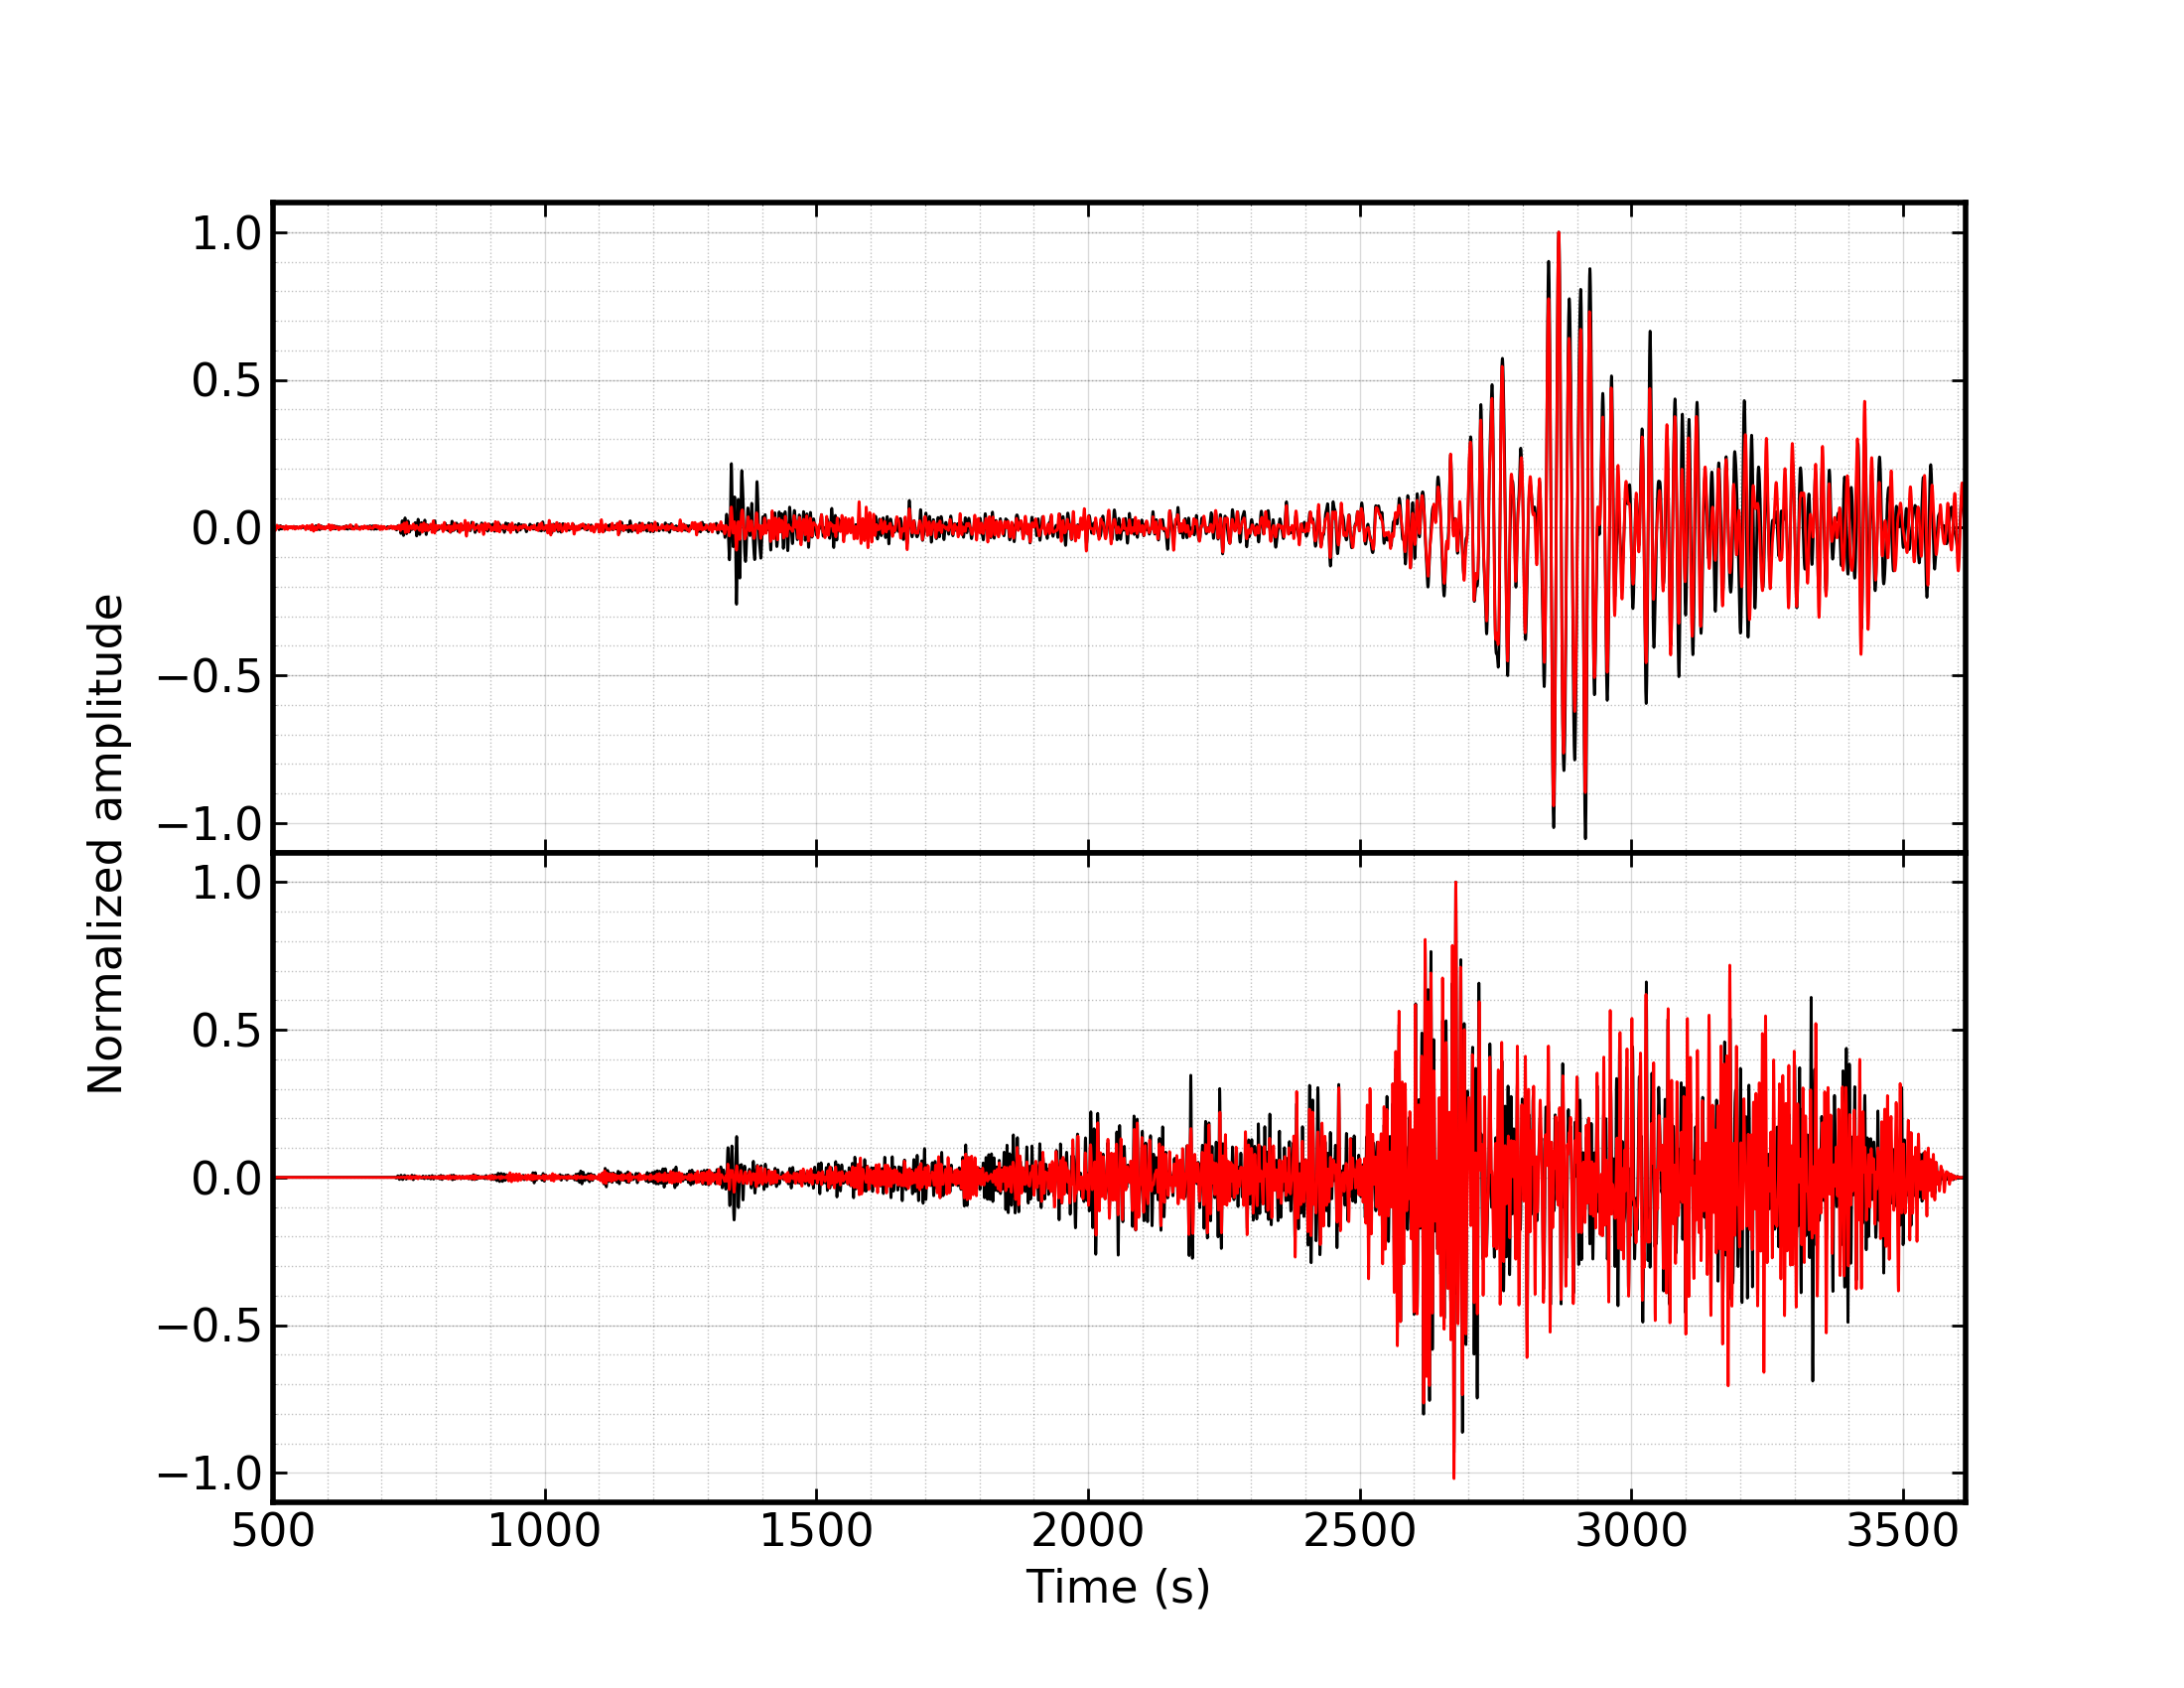
\includegraphics[width=0.5\textwidth]{C201109161926A_phmatch}}
\caption{Comparisons of rotation and translation. Observation (top) and synthetic (bottom) seismograms for an M$_w$ 6.67 event near Japan (see Table \ref{tab:syn_events}) . Waveforms filtered at 5 to 60 seconds. Red traces show rotation rate, black traces show transverse acceleration, amplitudes normalized from zero to one. Calculating for horizontal phase velocity with peak amplitudes using Equation \ref{eq:phasevelocity} gives c$_{obs}$ = 3.52 and c$_{syn}$ = 3.95 for observations and synthetics, respectively.}
\label{fig:rr_ta}
\end{figure}

\subsubsection{Peak correlation coefficient}
Correlations are a useful measure of similarity between two signals. It has been shown previously that for collocated measurements of vertical rotation rate and transverse acceleration, high values ($>0.9$) of zero lag correlations can be obtained in time windows centered around S-wave, or surface wave, arrivals \cite{igel2007broad}.
Zero lag correlation coefficients are routinely computed for events measured by G \cite{salvermoser2017event},
and are used in this study as a filtering tool to highlight "bad" events that exhibit low signal to noise ratios, or dissimilar waveforms which may arise due to non-physical effects (e.g. instrumental effects). Here, the largest correlation coefficient obtained for a seismogram is labeled the peak correlation coefficient (PCC), and is used as a representation of data quality.


\subsection{Magnitude scales}
Amplitude based magnitude scales provide empirically derived relationships between maximum trace amplitudes and source-receiver distances. Magnitude scales offer useful and quick estimates of relative sizes of earthquakes in a simple, standard  manner. 
The International Association of Planets Seismology and Earths Interior (IASPEI) Working Group on Magnitudes proposed a modified version of the original surface wave magnitude equation (Prague formula), proposed by \cite{karnik1962standardization}.
This broad band surface wave magnitude equation is compatible for use with modern day broadband seismic instruments \cite{bormann2000new}.

In this work, we adhere strictly to the standard procedures provided by IASPEI (outlined in the folllowing section) as a stencil for defining our own empirical magnitude scales. In turn, we use these derived scales as a tool for quantifying amplitude decay for different measured observables.

\subsubsection{Standard Procedures}\label{standproc}
The Working Group on Magnitudes' standard procedures gives the revised surface wave magnitude equation for broad-band instruments as,
\begin{equation}\label{eq:mag}
	M_S^{BB} = log_{10}(V/2\pi) + B\cdot log_{10}(\Delta) + C, 
\end{equation}
where the constants $B=1.66$ and $C=0.3$ control amplitude decay and order of magnitude, respectively. The parameter V should be the maximum trace amplitude (in nanometers second$^{-1}$) in the surface wave train, for a seismogram proportional to velocity, measured on the vertical component. 

Further criteria given by IASPEI posit that the period of the surface wave should lie within 3 s $\le$ T $\le$ 60 s, while epicentral distances should be between 2$^\circ \le \Delta \le 160^\circ$. It is further recommended that only shallow focus earthquakes should be considered, as medium to deep events are less capable of generating strong surface waves.
Maximum trace amplitudes are described as one half the largest peak to adjacent trough deflection, and associated period are given as two times the temporal difference between peak and adjacent trough. All events and processing steps in this paper adhere to these guidelines.

\subsubsection{Instrumental proxies for Love and Rayleigh waves}\label{proxy}
A standard procedure for determining surface wave magnitude scales is to take amplitudes measured on the vertical component of translation. This is because vertical translation should only be sensitive to the vertical motions of Rayleigh waves, whereas vector sums of horizontal components can be influenced by both Love and Rayleigh waves. In the same vein, velocity measured on the transverse component should only show sensitivity to Love waves (and radial components should only be sensitive to the horizontal component of Rayleigh waves). It is not common practice to use transverse components in calculating magnitude, due to the necessity of rotating horizontal components to the correct azimuth, which can be affected by ray paths, local site effects and correct epicenter location. The G-ring, which is 1) insensitive to translations and 2) proportional in phase and amplitude to transverse acceleration, should only be sensitive to Love waves in the surface wave train, irrespective of azimuth.  

In this study we use our instruments as physical wave-filters, in order to study individual phases in the surface wave train. This allows us to analyze the influences of Love waves and Rayleigh waves separately. By comparing the vertical and transverse components of translations, to the vertical component of rotation, we can understand, by proxy, the wave types they are sensitive to.

\subsubsection{Application of rotations to magnitude scales}
In order to give a fair comparison to translations using derived magnitude scales, a rotation parameter complementary to velocity is necessary. In Section \ref{phasevel}, an equation is given that relates rotation rates $\Omega$ with accelerations $\ddot{u}$. It would make the most sense, then, to compare velocities $\dot{u}$ with rotations $\omega$ (by integrating both sides). However, without previous work to draw precedence from, and for completeness, we present observations of both rotations and rotation rates in this study.

\section{Event choice}
The G-ring has been continuously recording at its current resolution since May, 2009 \cite{salvermoser2017event}. 
Events used in this study span from June 1, 2009 to September 1, 2016. An initial earthquake catalog was fetched from the Harvard Global Centroid Moment Tensor (GCMT) \cite{ekstrom2012global},
with events filtered by acceptable magnitude, source depth and epicentral distance from Wettzell, Germany. At this point we imposed the restriction that the derived 
"magnitude" as given by our magnitude equations, should fall as close to the given surface wave magnitude as possible. This ensures that our derived scales do not stray too far from established scales. Consequently we only consider events with published centroid moment magnitude values of $6 \le M_{\text{wc}} < 8$; surface wave magnitude and moment magnitude are approximately equal in this range \cite{shearer2009introduction}.
 Zero-lag cross correlations of transverse acceleration and rotation rate were taken in order to calculate peak correlation coefficients (Section \ref{sec:dataproc}). Events were not considered if their peak correlation coefficient did not meet the criterion PCC $\geq 0.7$. 

These choices for event criteria narrowed the catalog down to roughly 500 events. Each event was appropriately filtered and processed (Section \ref{sec:dataproc}), and waveforms were individually inspected. Waveforms that exhibited anomalous behavior (e.g. unexpected high amplitude peaks outside the surface wave train, high signal-to-noise ratio etc.) were rejected. A final event catalog of 243 events was reached, shown in Figure \ref{fig:event_map}.

\begin{figure*}
\centerline{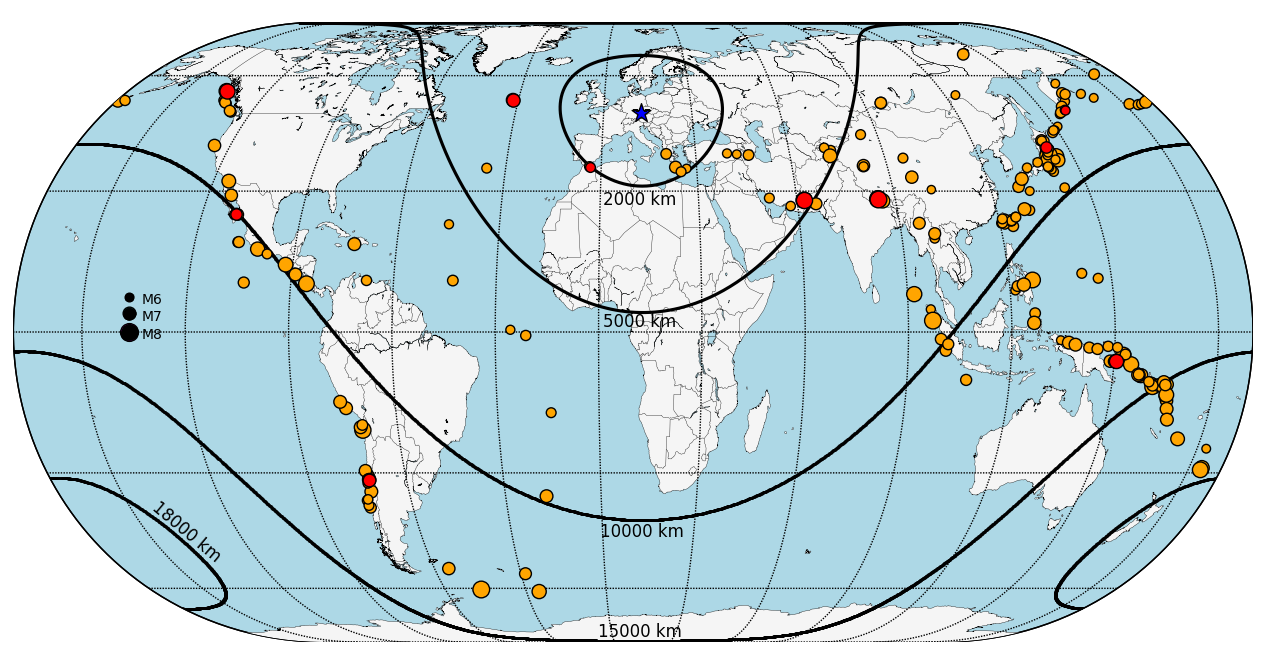
\includegraphics[width=.8\textwidth]{event_map}}
\caption{Event map. Size represents moment magnitude (M$_{wc}$). Orange dots show observed earthquakes used in magnitude scale derivation. Red dots show the ten events chosen for generation of synthetic seismograms. Black lines are equidistant points from the blue star, which represents the location of G in Wettzell, Germany (49.144$^\circ$N,12.87$^\circ$E).}
\label{fig:event_map}
\end{figure*}

\section{Methods}
\subsection{Data Processing}\label{sec:dataproc}
Events were processed in a similar fashion as the processing outlined in Salvermoser et al. \shortcite{salvermoser2017event}. 
Raw, continuous translation data in North, East and vertical components, as well as vertical rotation rate data, was fetched based on event origin time. Instrument response correction produced translation seismograms proportional to units of velocity (nm s$^{-1}$). Epicentral distances ($\Delta$) and theoretical backazimuth values were calculated from station-receiver latitude longitude pairs, and events were separated into categories of close ($\Delta < 3^\circ$), local ($\Delta <100^\circ$) and far ($\Delta \ge 100^\circ$). Translations were rotated into the transverse, radial, vertical coordinate system by the appropriate theoretical backazimuth. Measurements from ring laser gyroscope instruments do not require frequency dependent instrument correction \cite{schreiber2006ring},
therefore only a simple scale factor was necessary to retrieve seismograms proportional to rotation rate (nrad s$^{-1}$). 

Rotation rate traces were integrated to provide measurements of rotation (nrad), and transverse velocity was integrated to retrieve transverse acceleration, which was subsequently used to calculate correlations with vertical rotation rates.
A bandpass filter was applied to all traces for periods between 3 s $\le$ T $\le$ 60 s, in accordance to the IASPEI standard procedures. Peak amplitudes were chosen by finding minimum and maximum trace values and the largest associated peak or trough, respectively. The larger of the two was recorded, alongside the associated arrival time and dominant period, taken as two times the distance between peak and adjacent trough. 

Theoretical considerations were initially used to restrict search to the surface wave train, however results proved inconsistent, so maximum amplitudes in the entire trace were considered. Through manual inspection, picked amplitudes that fell outside the surface wave train (which occurred very infrequently) were rejected. An example of the waveform and amplitude picking is shown in Figure \ref{fig:obswav}.


\begin{figure}
\centerline{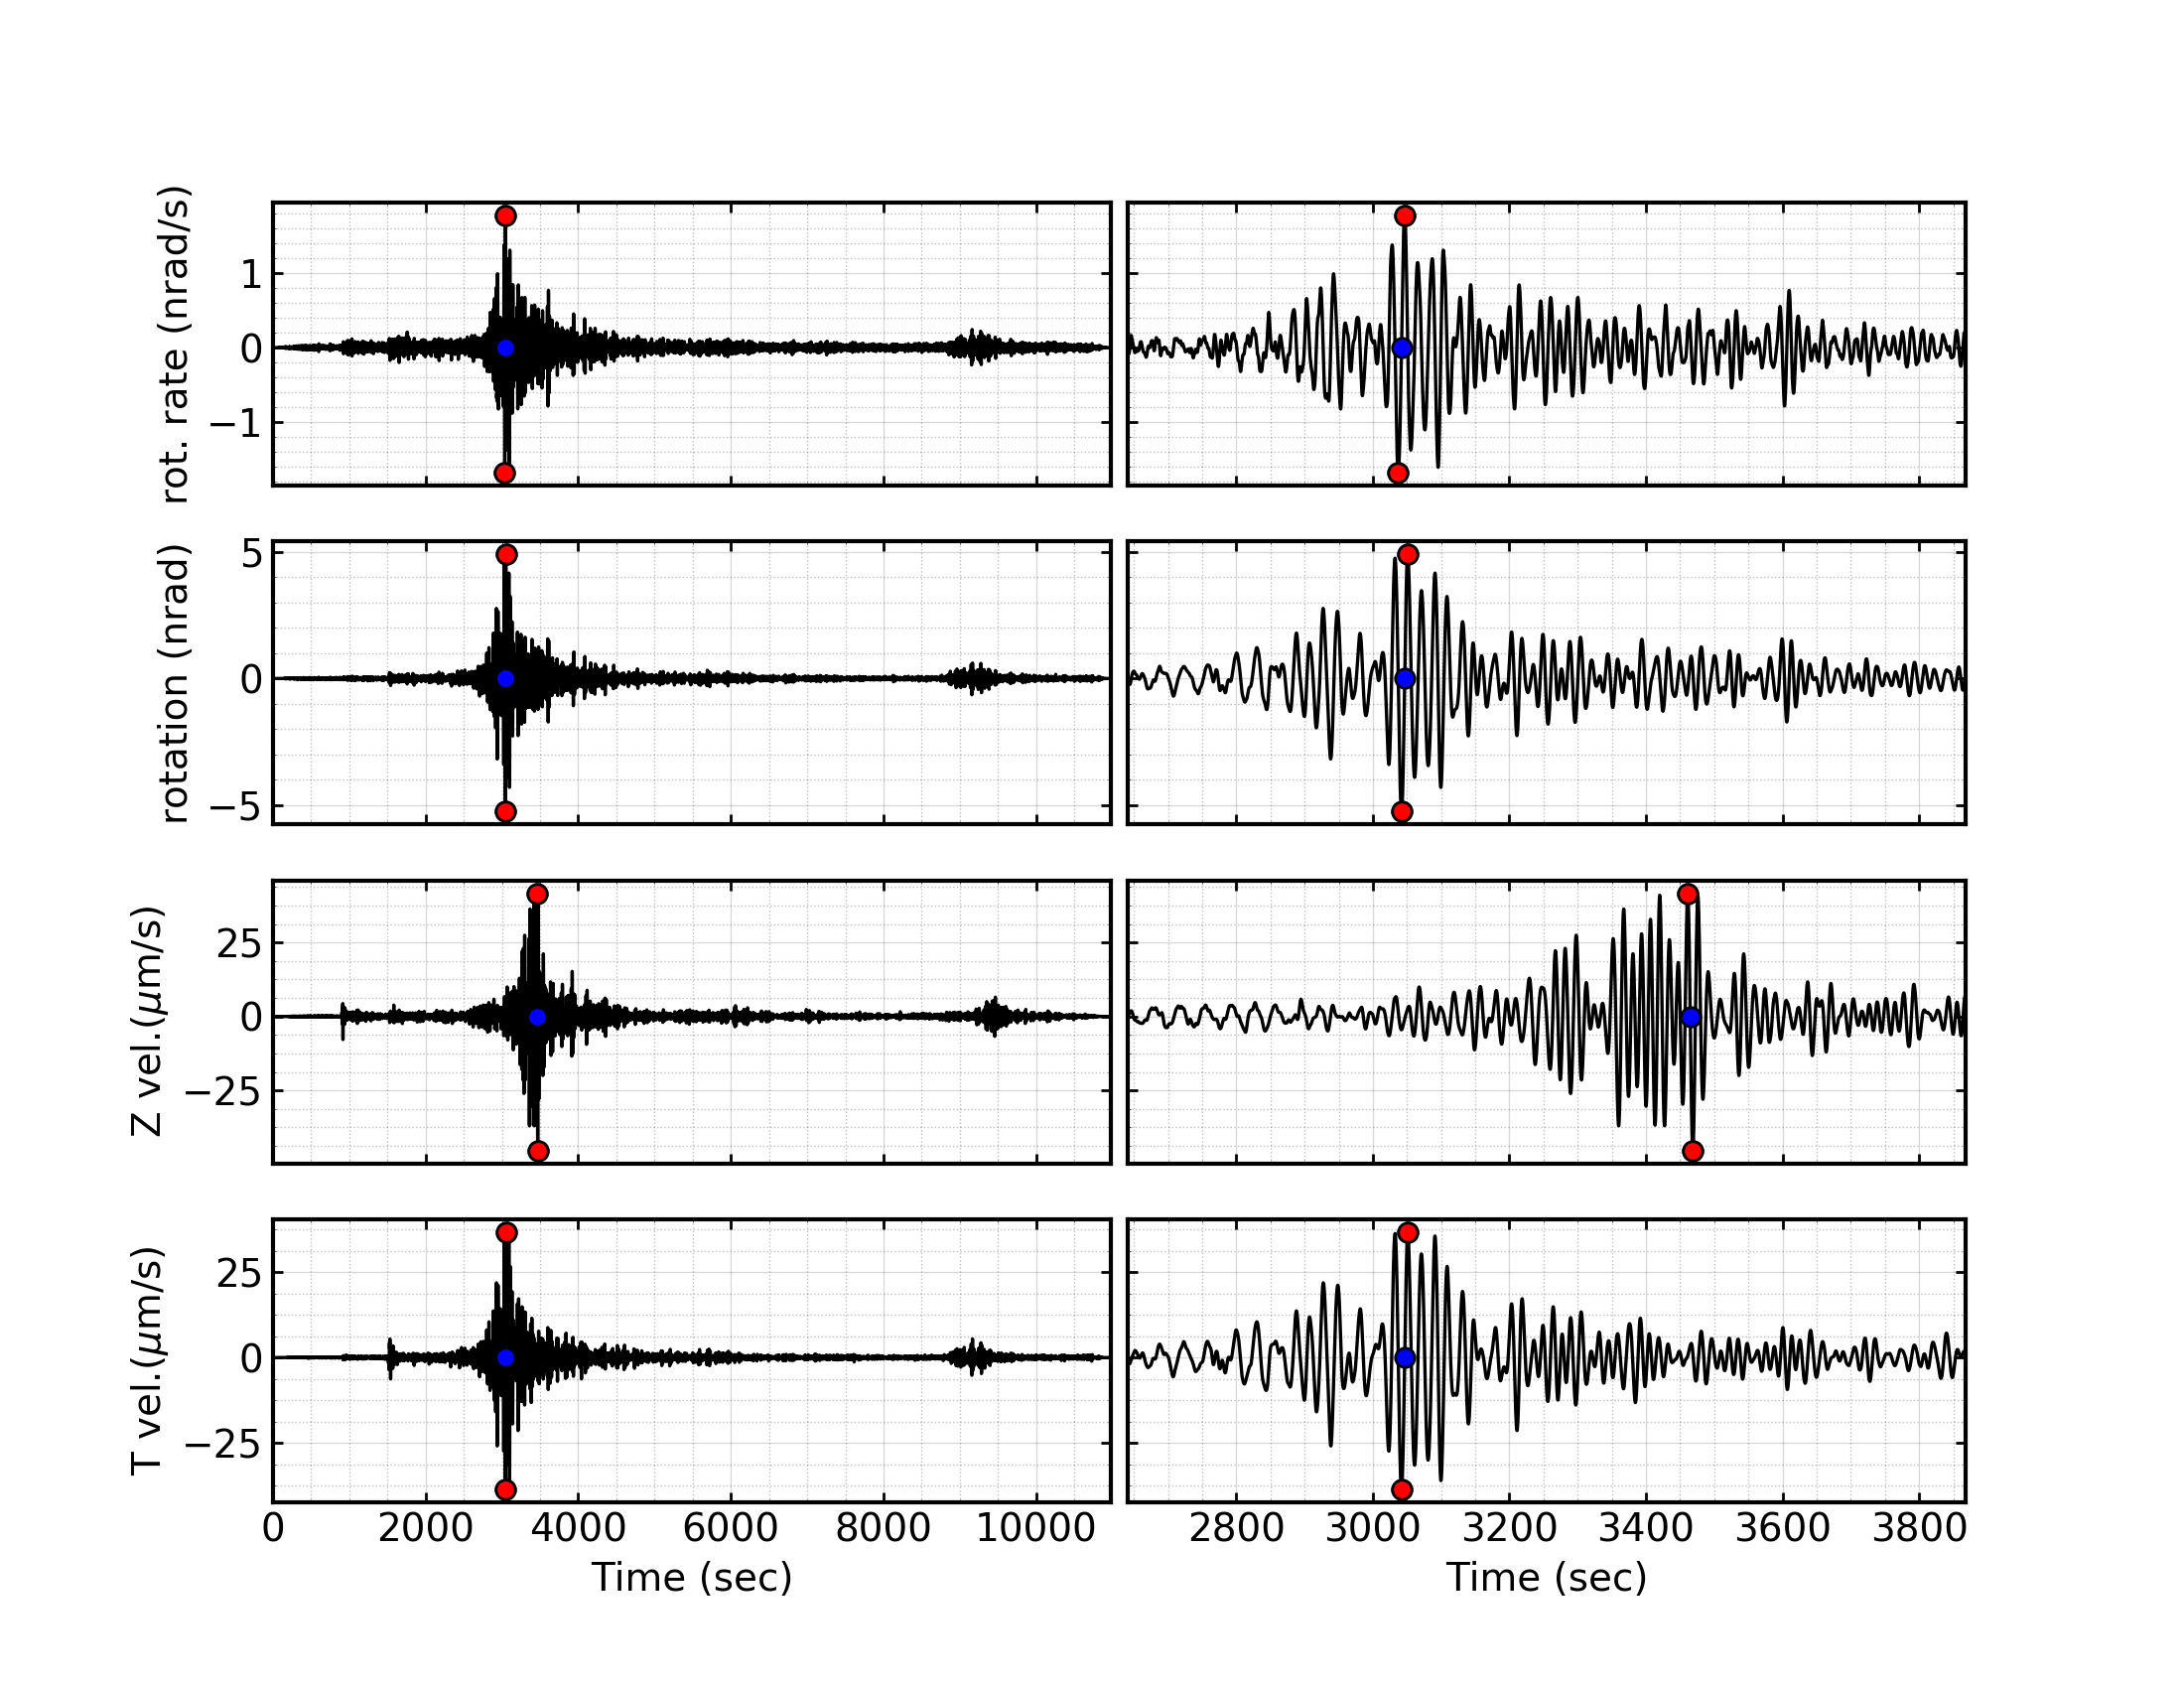
\includegraphics[width=0.5\textwidth]{amp_picking_update-2011-09-16}}
\caption{Peak amplitude picking. Left column shows seismograms of the 2011 M$_w$ 6.67 event (See Table \ref{tab:syn_scales}). From top to bottom: rotation rate, rotation, vertical velocity, transverse velocity. Red dots show largest peak to peak. Blue dots shows zero crossing for the chosen peak to peak amplitude. \newline Right column shows zoomed in section of respective seismograms. Note the visible difference in amplitude picks of the Love wave and the later arriving Rayleigh wave.}
\label{fig:obswav}
\end{figure}


\subsubsection{Zero-lag correlations}
To calculate peak correlations, traces of transverse acceleration and vertical rotation rate were segmented into small time windows based on the event-station distance. In each time window, a zero-lag correlation was performed, and a single value of correlation produced. From the entire trace, the max value was taken to represent the peak correlation coefficient. For most waveforms, the peak correlation coefficient lies in the surface wave train. As mentioned previously, these peak correlation values are used extensively as a ranking system for events, providing a quickly attainable measure of waveform quality.

\subsection{Curve fitting}
To quantify amplitude decay, magnitude scale coefficients were fit to the data using a simple linear regression. Using the general form of the magnitude equation, given by Equation \ref{eq:mag}, a collection of $n$ events can be represented in the form, 
\begin{equation}
	\begin{pmatrix}
		log_{10}(\Delta_{1}) & 1 \\
		log_{10}(\Delta_{2}) & 1 \\
		\vdots  & \vdots \\
		log_{10}(\Delta_{n}) & 1 
	\end{pmatrix}
	\begin{pmatrix}
		{B}\\
		{C}
	\end{pmatrix}
	=
	\begin{pmatrix}
		M_{\text{wc}_1} - log_{10}({V_1}/{2\pi})_{\text{max}} \\
		M_{\text{wc}_2} - log_{10}({V_2}/{2\pi})_{\text{max}} \\
		\vdots  \\
		M_{\text{wc}_n} - log_{10}({V_n}/{2\pi})_{\text{max}}
	\end{pmatrix},
	\label{eq:linearreg}
\end{equation}

\noindent which can be expressed in the matrix-vector form, $\mathbf{Gm = d}$. The unknowns B and C are represented in the vector {\bfseries m}, and can be solved for through the normal equation $\mathbf{m} = \mathbf{(G}^{T}\mathbf{G})^{-1}\mathbf{G}^T\mathbf{d}$. By solving for the vector $\mathbf{m}$, we create an empirical magnitude scale that best describes the amplitude decay behavior of our observations. In Equation \ref{eq:linearreg}, we impose that our derived magnitude value should be as close to the given moment magnitude as possible, by setting $M_S^{BB}$ equal to the value of $M_\text{wc}$ retrieved from our event catalog. 

Confidence intervals were constructed for each parameter of the vector $\mathbf{m}$. These were calculated with the variance of estimates of the $j$th parameter of $\mathbf{m}$ by the equation $\hat{m}_j \pm c \sqrt{\hat{var}(\hat{m}_j)}$, where the value of c is given as 1.96 for a confidence interval of $\alpha = 0.95$. [more explanation of confidence intervals needed]

\section{Synthetic seismograms}
Due to the unique instrumental setup of the G-ring, there are currently no other datasets to draw comparisons against. It should be mentioned that there are other available rotation instruments which have been used for earthquake analyses \cite{donner2017comparing}, \cite{sbaa2017analysis}, however they lack any substantial earthquake catalog. One possibility for gathering more observations would be through array derived rotations as a substitute for direct rotation measurements; this option was noted during analysis, however it proved difficult finding sufficient long-term arrays with optimal station spacing. If this type of data became available or accessible, it would provide a very useful addition of information. In lieu of this, we turn to waveform modeling to generate synthetic seismograms, with which we recreate our experimental setup to provide a comparable set of synthetic observations.

The seismic wave propagation code Specfem3D Globe was employed. A realistic global model featuring 3D crust (crust2.0 \cite{Bassin2000}) and mantle (S40RTS \cite{Ritsema2011}) models was used. The simulation featured effects that might have potential influence on surface waves at the periods of interest, which include: ocean loading, Earth ellipticity, topography, self gravitation, Earth's rotation and 1-D attenuation. Event locations and moment tensors were taken from 10 real seismic events present in the observation catalogs. Events were chosen based on values of peak correlation coefficients, as well as optimal event location and depth, so as to provide a varied distribution of source-receiver pairings. Table \ref{tab:syn_events} provides detailed information on the chosen events. 

In each simulation, events were initiated as point sources. The simulation corner frequency was set to 10 seconds, and simulations were run for one hour simulation time. As computational cost is independent of number of stations, more than one hundred stations were included; station locations were taken from Global Seismic Network (GSN) locations,with the addition of the G-ring, and the German observatory station F\"urstenfeldbruck (48.163$^\circ$N, 11.275$^\circ$E), which was used for comparisons in observations.

\begin{table*}
\begin{minipage}{150mm}
	\begin{center}
		\begin{tabular}{ |c|c|c|c|c|c|c|c| } 
		\bf{Date} & \bf{Time (UTC)} & \bf{Lat($^\circ$)} & \bf{Lon($^\circ)$} & \bf{Depth(km)} & \bf{$\Delta$ ($^\circ$)} & \bf{M$_{\text{wc}}$} &\bf{Flinn-Engdahl Region} \\ \hline
	2010-07-18 & 13:34:59 & -5.93 & 150.59 & 35.0 & 124.3 & 7.32 & New Britain Region, P.N.G. \\
	2011-09-16 & 19:26:41 & 40.27 & 142.78 & 35.0 & 80.8 &  6.67 & Off East Coast Of Honshu, Japan \\
	2013-01-05 & 08:58:19 & 55.39 & -134.65 & 10.0 & 72.1 & 7.53 & Southeastern Alaska \\
	2013-04-16 & 10:44:20 & 28.03 & 62.0 & 80.0 & 43.2 & 7.74 & Southern Iran \\
	2013-04-19 & 19:58:40 & 49.97 & 157.65 & 15.0 &76.8 & 6.06 & East Of Kuril Islands \\
	2015-02-13 & 18:59:12 & 52.65 & -31.9 & 16.7 & 28.6 & 7.07 & Reykjanes Ridge \\
	2015-04-25 & 06:11:26 & 28.15 & 84.71 & 15.0 & 58.3 & 7.88 & Nepal \\
	2015-09-13 & 08:14:12 & 25.14 & -109.43 & 10.0 & 90.1 & 6.6 & Gulf Of California \\
	2015-09-16 & 23:18:41 & -31.56 & -71.43 & 28.4 & 110.3 & 7.1 & Near Coast Of Central Chile \\
	2016-01-25 & 04:22:02 & 35.65 & -3.68 & 12.0 & 18.2 & 6.38 & Strait Of Gibraltar \\
		\end{tabular}
    		\caption{List of events used as synthetic sources in Specfem3D. Events were chosen based on a diverse coverage of magnitudes and epicentral distances ($\Delta$) from the ring laser stationed in Wettzell, Germany. Event information taken from the GCMT catalog.}
		\label{tab:syn_events}
	\end{center}
	\end{minipage}
\end{table*}

%\begin{table*}
%\begin{minipage}{150mm}
%	\begin{center}
%		\begin{tabular}{ |c|c|c|c|c|c|c|c|c| } 
%		\bf{Date} & \bf{Time (UTC)} & \bf{Lat($^\circ$)} & \bf{Lon($^\circ)$} & \bf{Depth(km)} & \bf{$\Delta$ ($^\circ$)} & \bf{M$_{\text{wc}}$} &\bf{Flinn-Engdahl Region} &\bf{Peak Corr. Coeff.}\\ \hline
%	2010-07-18 & 13:34:59 & -5.93 & 150.59 & 35.0 & 124.3 & 7.32 & New Britain Region, P.N.G. & 0.98\\
%	2011-09-16 & 19:26:41 & 40.27 & 142.78 & 35.0 & 80.8 &  6.67 & Off East Coast Of Honshu, Japan & 0.99\\
%	2013-01-05 & 08:58:19 & 55.39 & -134.65 & 10.0 & 72.1 & 7.53 & Southeastern Alaska & 0.95\\
%	2013-04-16 & 10:44:20 & 28.03 & 62.0 & 80.0 & 43.2 & 7.74 & Southern Iran & 0.98\\
%	2013-04-19 & 19:58:40 & 49.97 & 157.65 & 15.0 &76.8 & 6.06 & East Of Kuril Islands & 0.99\\
%	2015-02-13 & 18:59:12 & 52.65 & -31.9 & 16.7 & 28.6 & 7.07 & Reykjanes Ridge & 0.99\\
%	2015-04-25 & 06:11:26 & 28.15 & 84.71 & 15.0 & 58.3 & 7.88 & Nepal & 0.99\\
%	2015-09-13 & 08:14:12 & 25.14 & -109.43 & 10.0 & 90.1 & 6.6 & Gulf Of California & 0.98\\
%	2015-09-16 & 23:18:41 & -31.56 & -71.43 & 28.4 & 110.3 & 7.1 & Near Coast Of Central Chile & 0.99\\
%	2016-01-25 & 04:22:02 & 35.65 & -3.68 & 12.0 & 18.2 & 6.38 & Strait Of Gibraltar & 0.99\\
%		\end{tabular}
%    		\caption{List of events used as synthetic sources in Specfem3D. Peak correlations are used as a measure of waveform quality, and only events with the highest values were used, in order to provide the best comparisons of synthetics with observations. Events were also chosen based on a diverse coverage of magnitudes and epicentral distances from the ring laser stationed in Wettzell, Germany. Event information taken from the GCMT catalog.}
%		\label{tab:syn_events}
%	\end{center}
%	\end{minipage}
%\end{table*}

%The direct outputs of Specfem3D were adjusted to produce displacement (in units of meters) in the transverse, radial and vertical components, by rotation with respect to the theoretical backazimuth. Direct rotation (in units of radians) in the same coordinate system was also outputted. During processing, translation seismograms were differentiated to retrieve velocity waveforms, and rotation was differentiated to produce rotation rate waveforms. A work flow identical to that used for observations was employed to calculate peak trace amplitudes, and a magnitude equation was fit to the data for comparison.

\section{Results}\label{sec:results}
\subsection{Derived magnitude scales}
Decay characteristics of rotations and translations were derived by solving for B and C in Equation \ref{eq:linearreg}. The values for each scale are presented in Table \ref{tab:scales}. For an additional check on site-dependent data quality, the same analysis was performed on translation observations taken at the geophysical observatory F\"urstenfeldbruck, Germany (FUR; 48.163$^\circ$N, 11.275$^\circ$E), located roughly 200 km south-west of Wettzell, as well as for a station in Pi\~non Flats Observatory, California, USA. Though a smaller subset of events was used due to data availability, the results confirmed those given at Wettzell. 


\begin{figure*}
\centerline{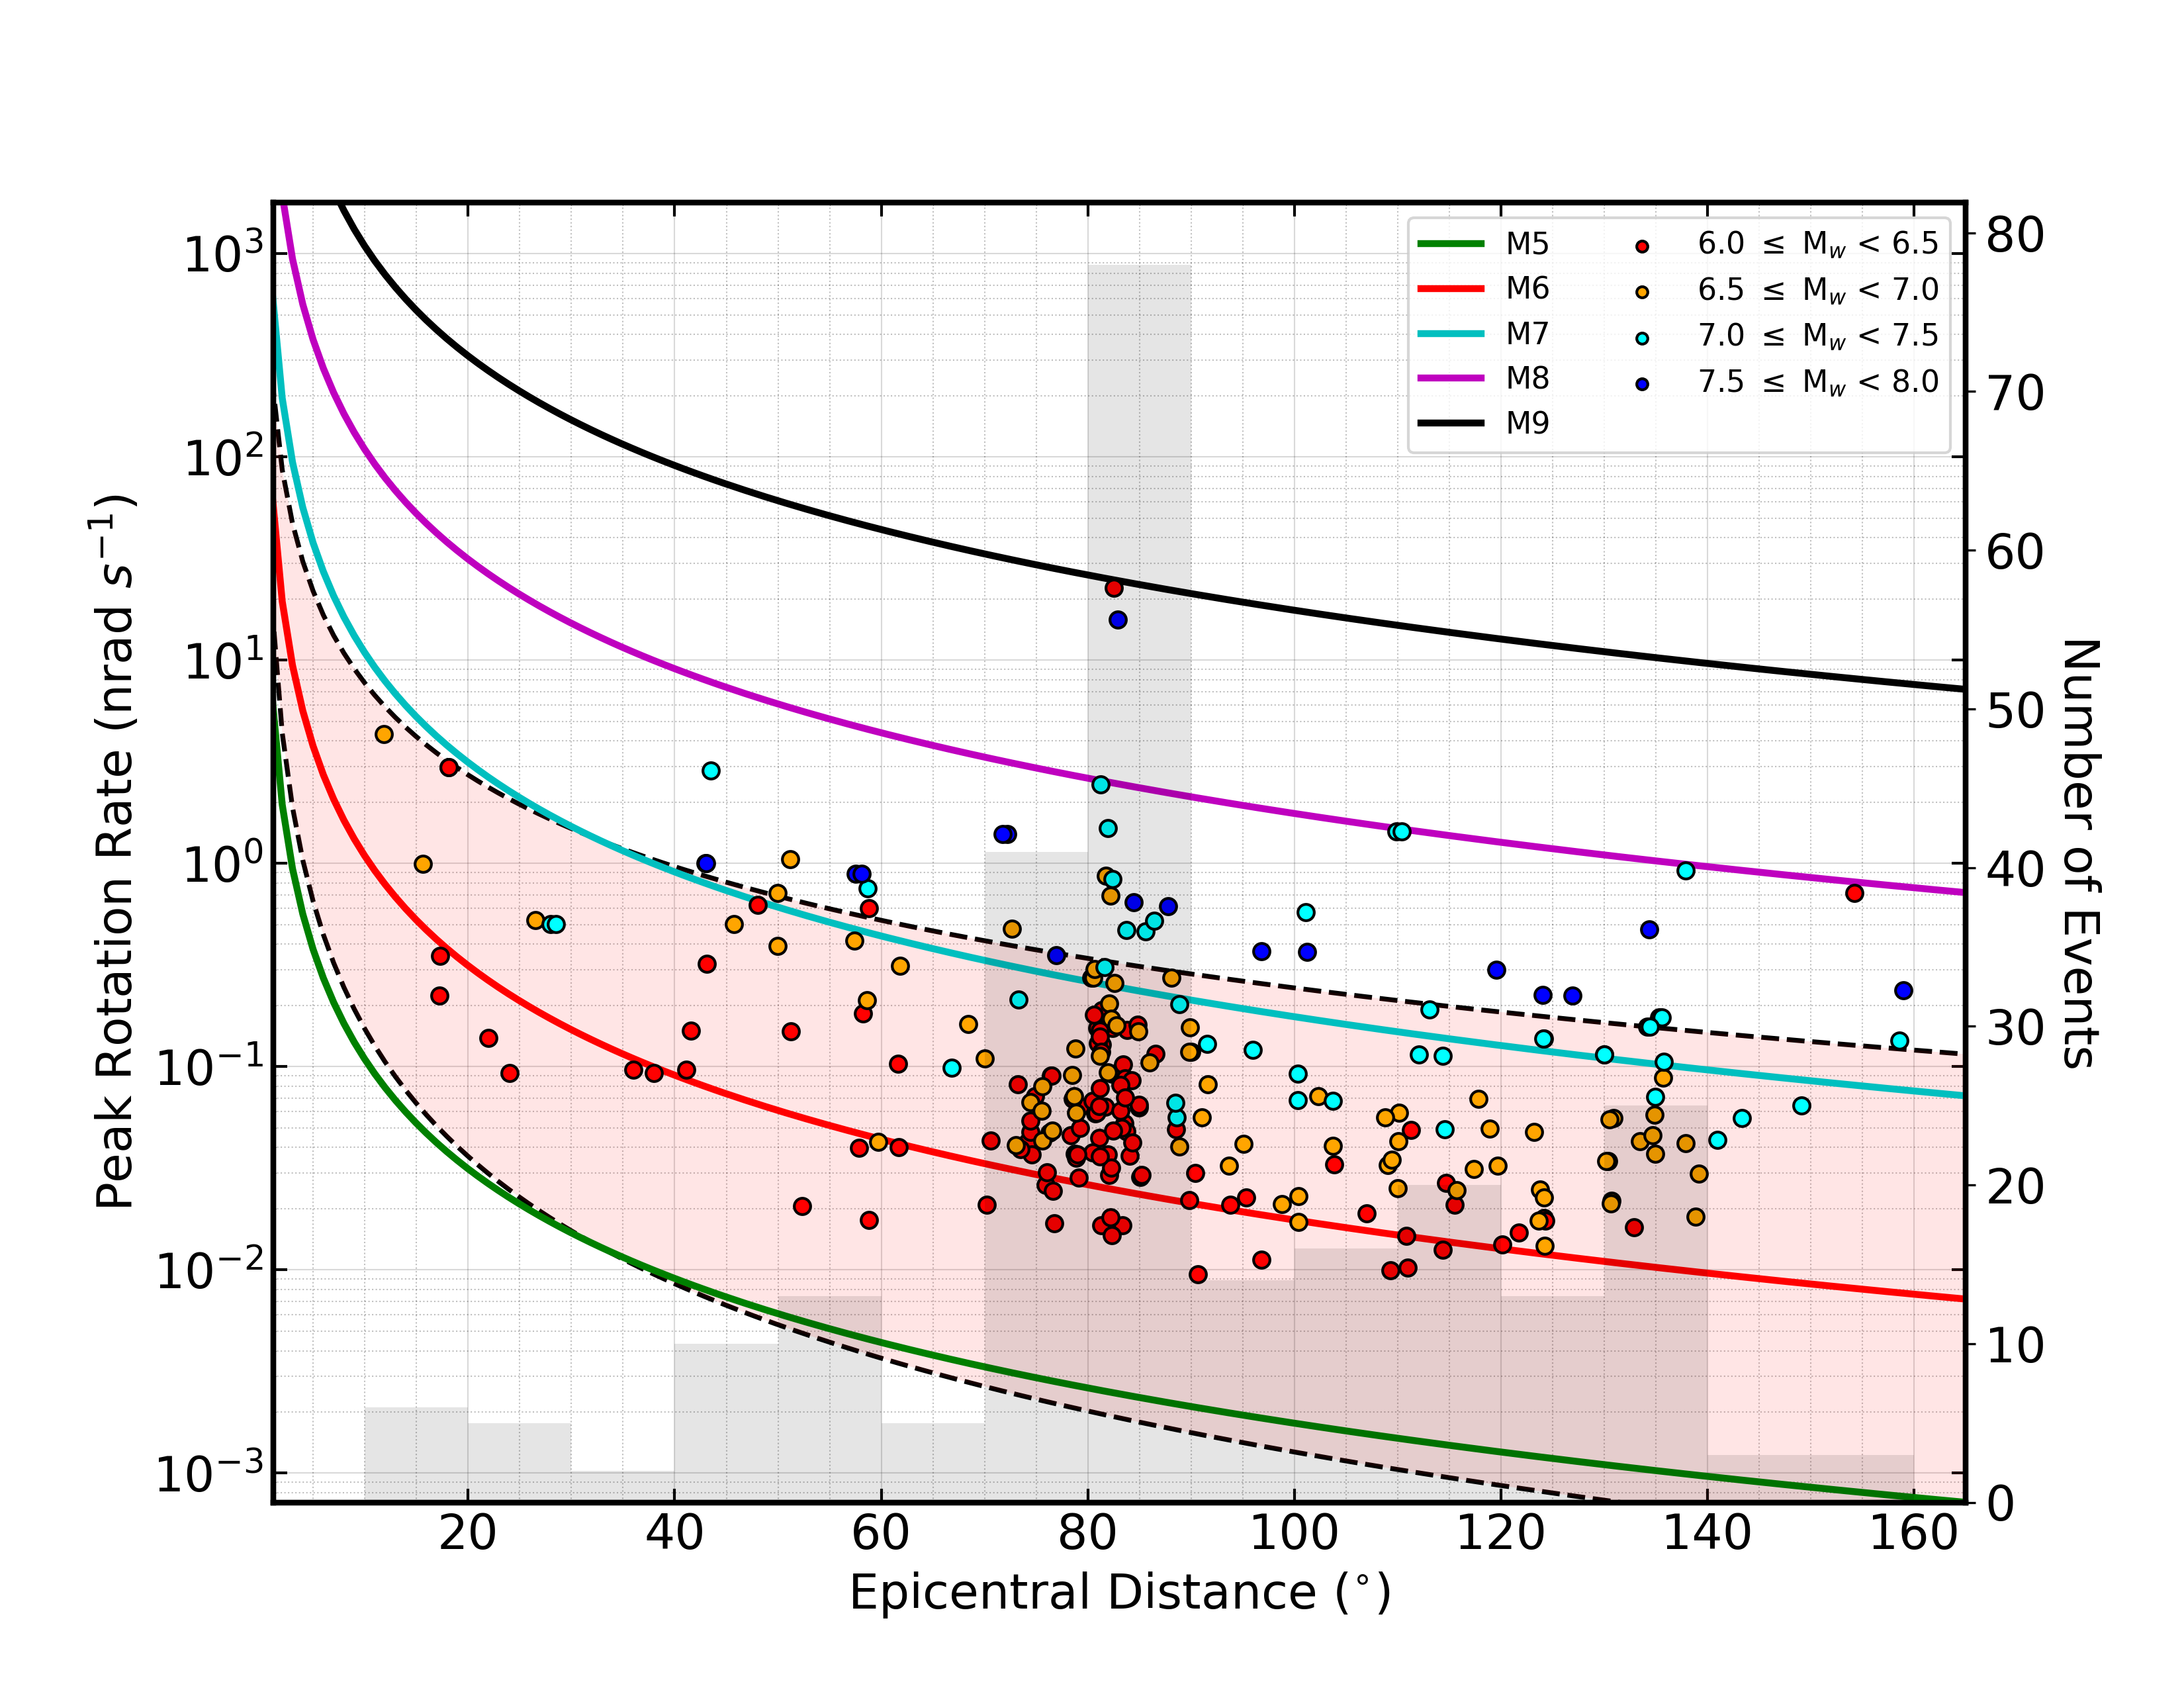
\includegraphics[width=1.0\textwidth]{RT_WET}}
\caption{Rotation rate magnitude scale for observations. Constants for decay lines are B=1.823, C=4.113. Event magnitudes separated by bins of 0.5 and denoted by color. Magnitude equation plotted by integer values as solid color lines. 95\% confidence interval for M6 shown by the shaded red area, bordered by black dashed lines. The number of events for each epicentral distance bin shown by gray bars in the background.}
\label{fig:rr_obs}
\end{figure*}

%translation scales
Derived values of B range from 1.084 to 1.823 for vertical velocity M$^{WET}_{Z}$ and rotation rate M$^{RLAS}_{RR}$, respectively. Rotation M$^{RLAS}_{RT}$ falls closest to the standard IASPEI value of 1.66. Velocity values are consistent between Wettzell and F\"urstenfeldbruck, with FFB showing slightly higher amplitudes, as seen in the value of C, which controls the order of magnitude of expected amplitudes. Larger amplitudes are visible in the transverse component of FFB relative to WET, seen in Figure \ref{fig:vel_scale}, however the vertical component does not reflect this. 

There exists a noticeable difference between values of B for transverse and vertical velocities. The vertical velocity scale is expected to present an identical setup to the broadband surface wave magnitude equation, however it presents the largest discrepancy, for both stations WET and FUR. Transverse velocity, which should sample Love waves, same as rotations (see \ref{proxy}), shows a larger value for B as compared to vertical velocity.

\begin{figure}
\centerline{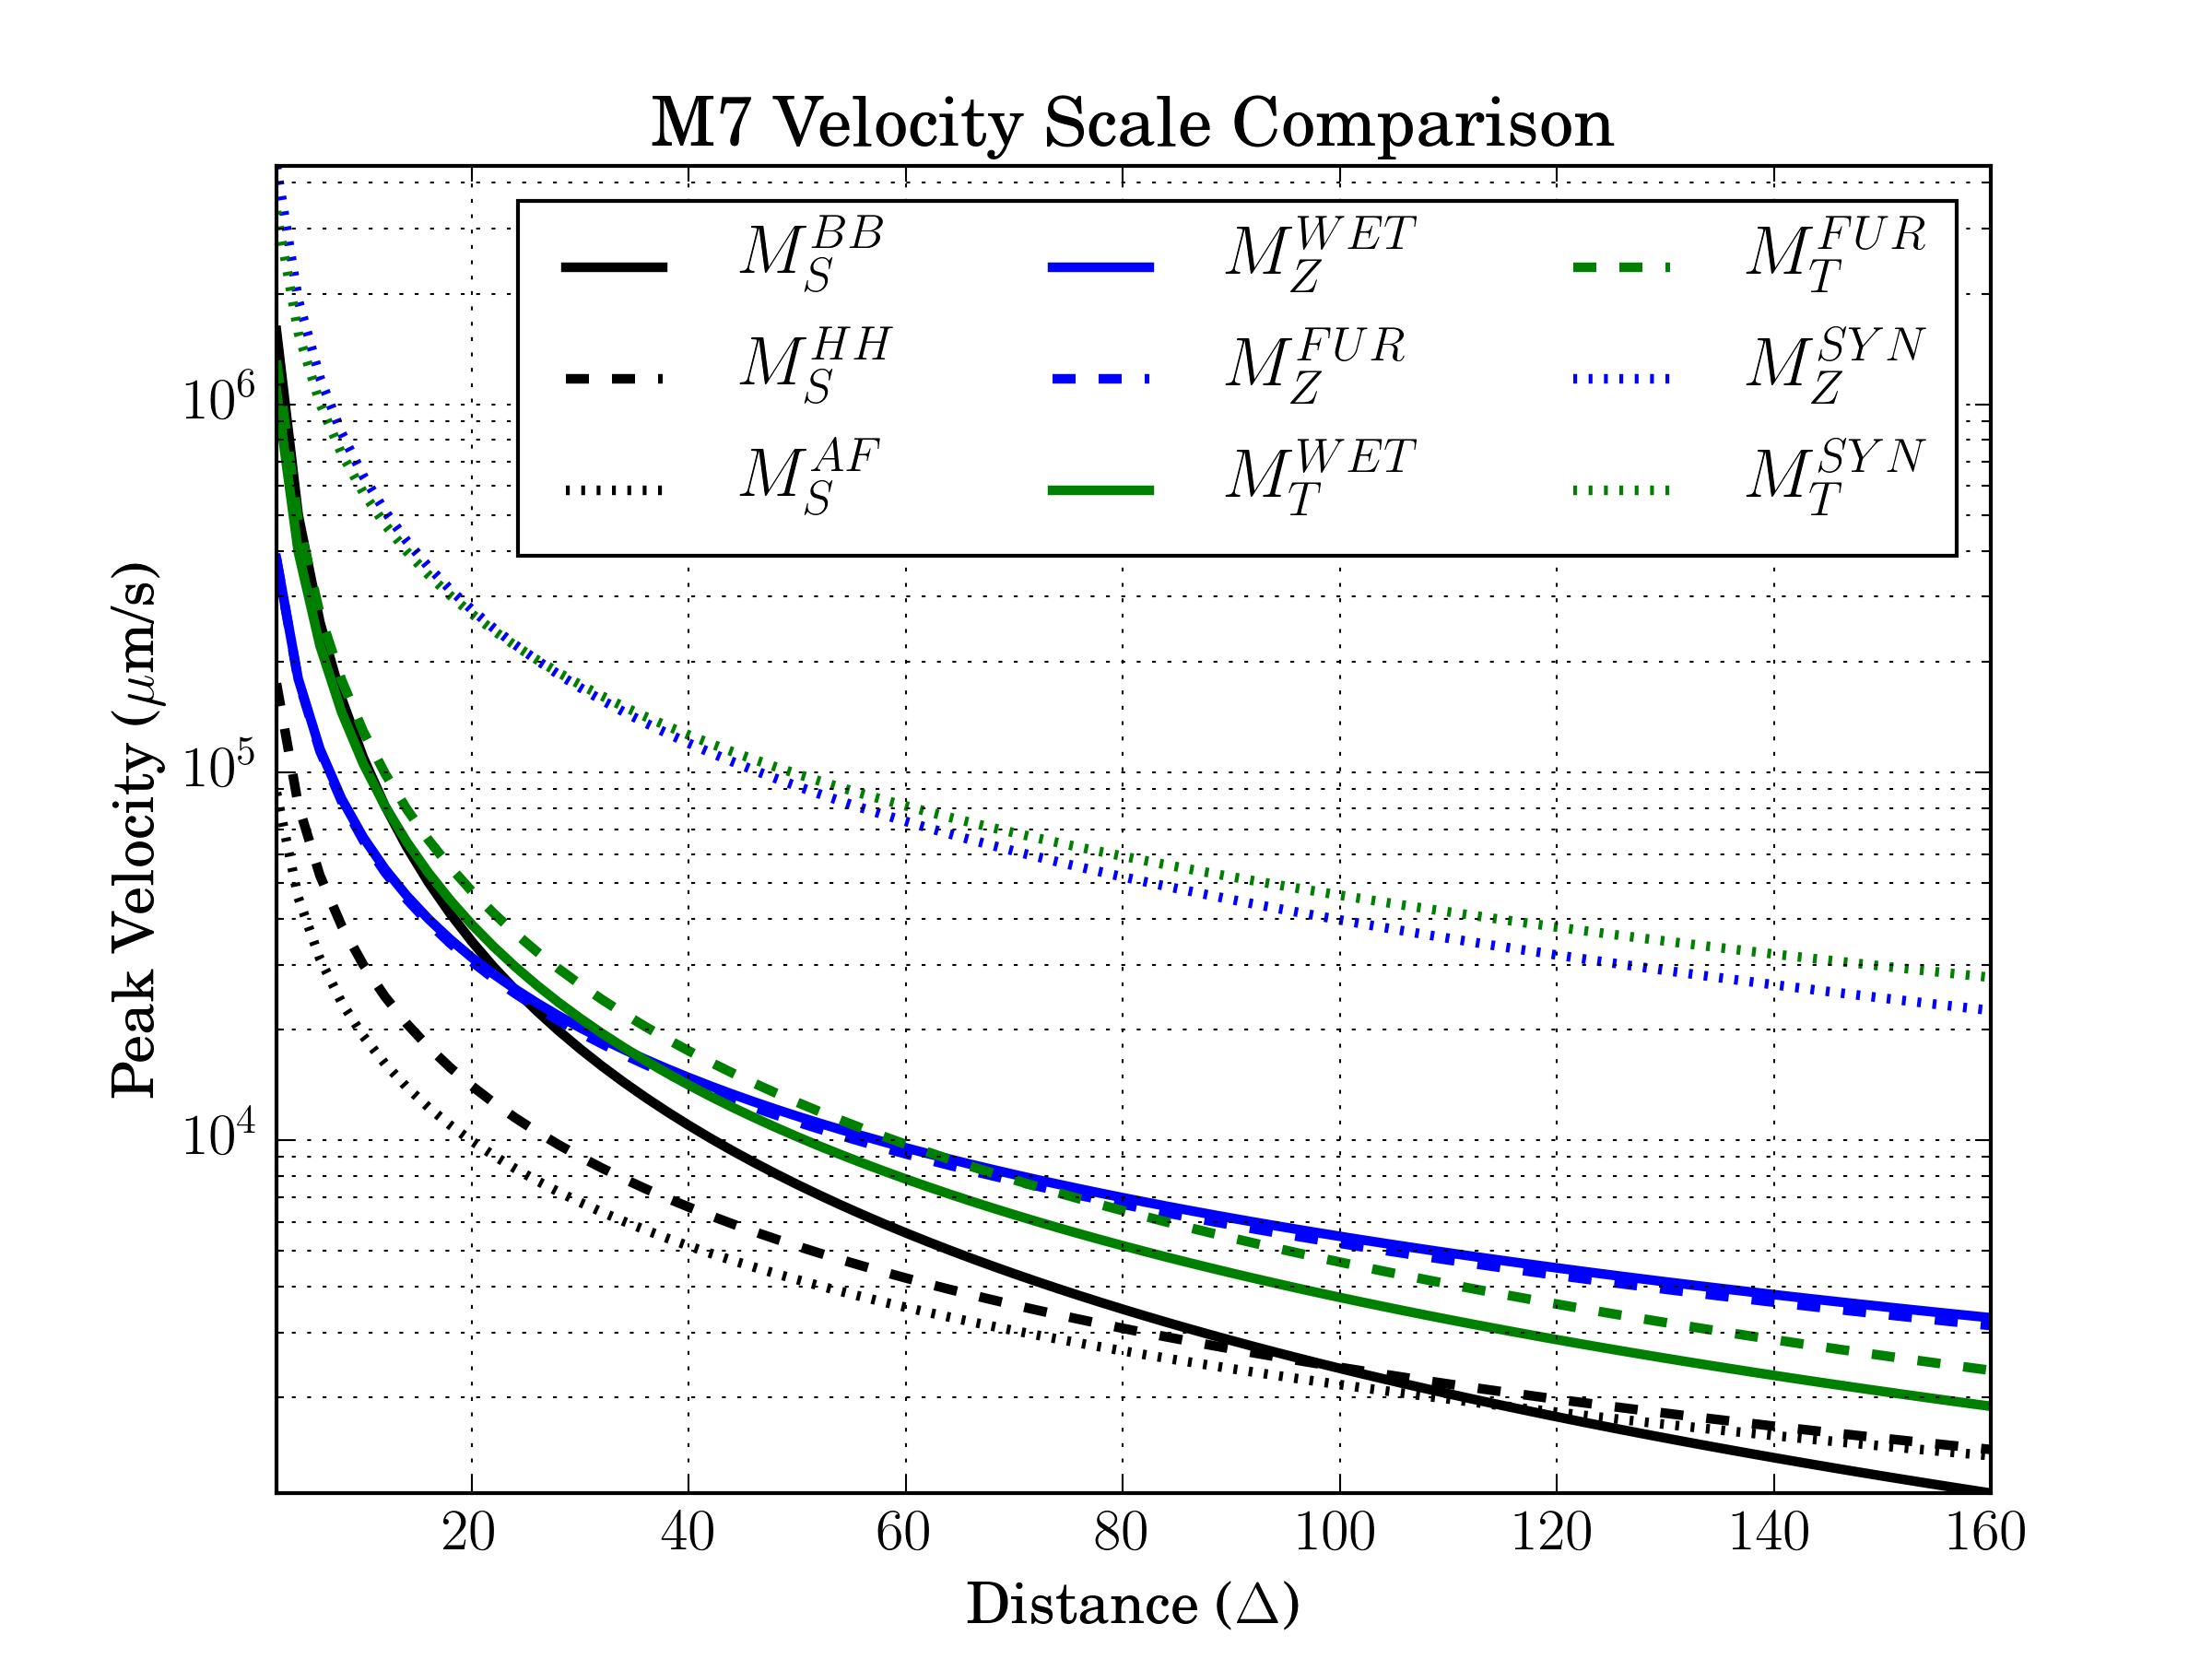
\includegraphics[width=.5\textwidth]{velocityscales}}
\caption{A comparison of velocity based scales for stations WET, FUR and synthetic scales, with the IASPEI scale used as reference. Peak amplitudes given in units of nanometers/s}
\label{fig:vel_scale}
\end{figure}

\begin{figure}
\centerline{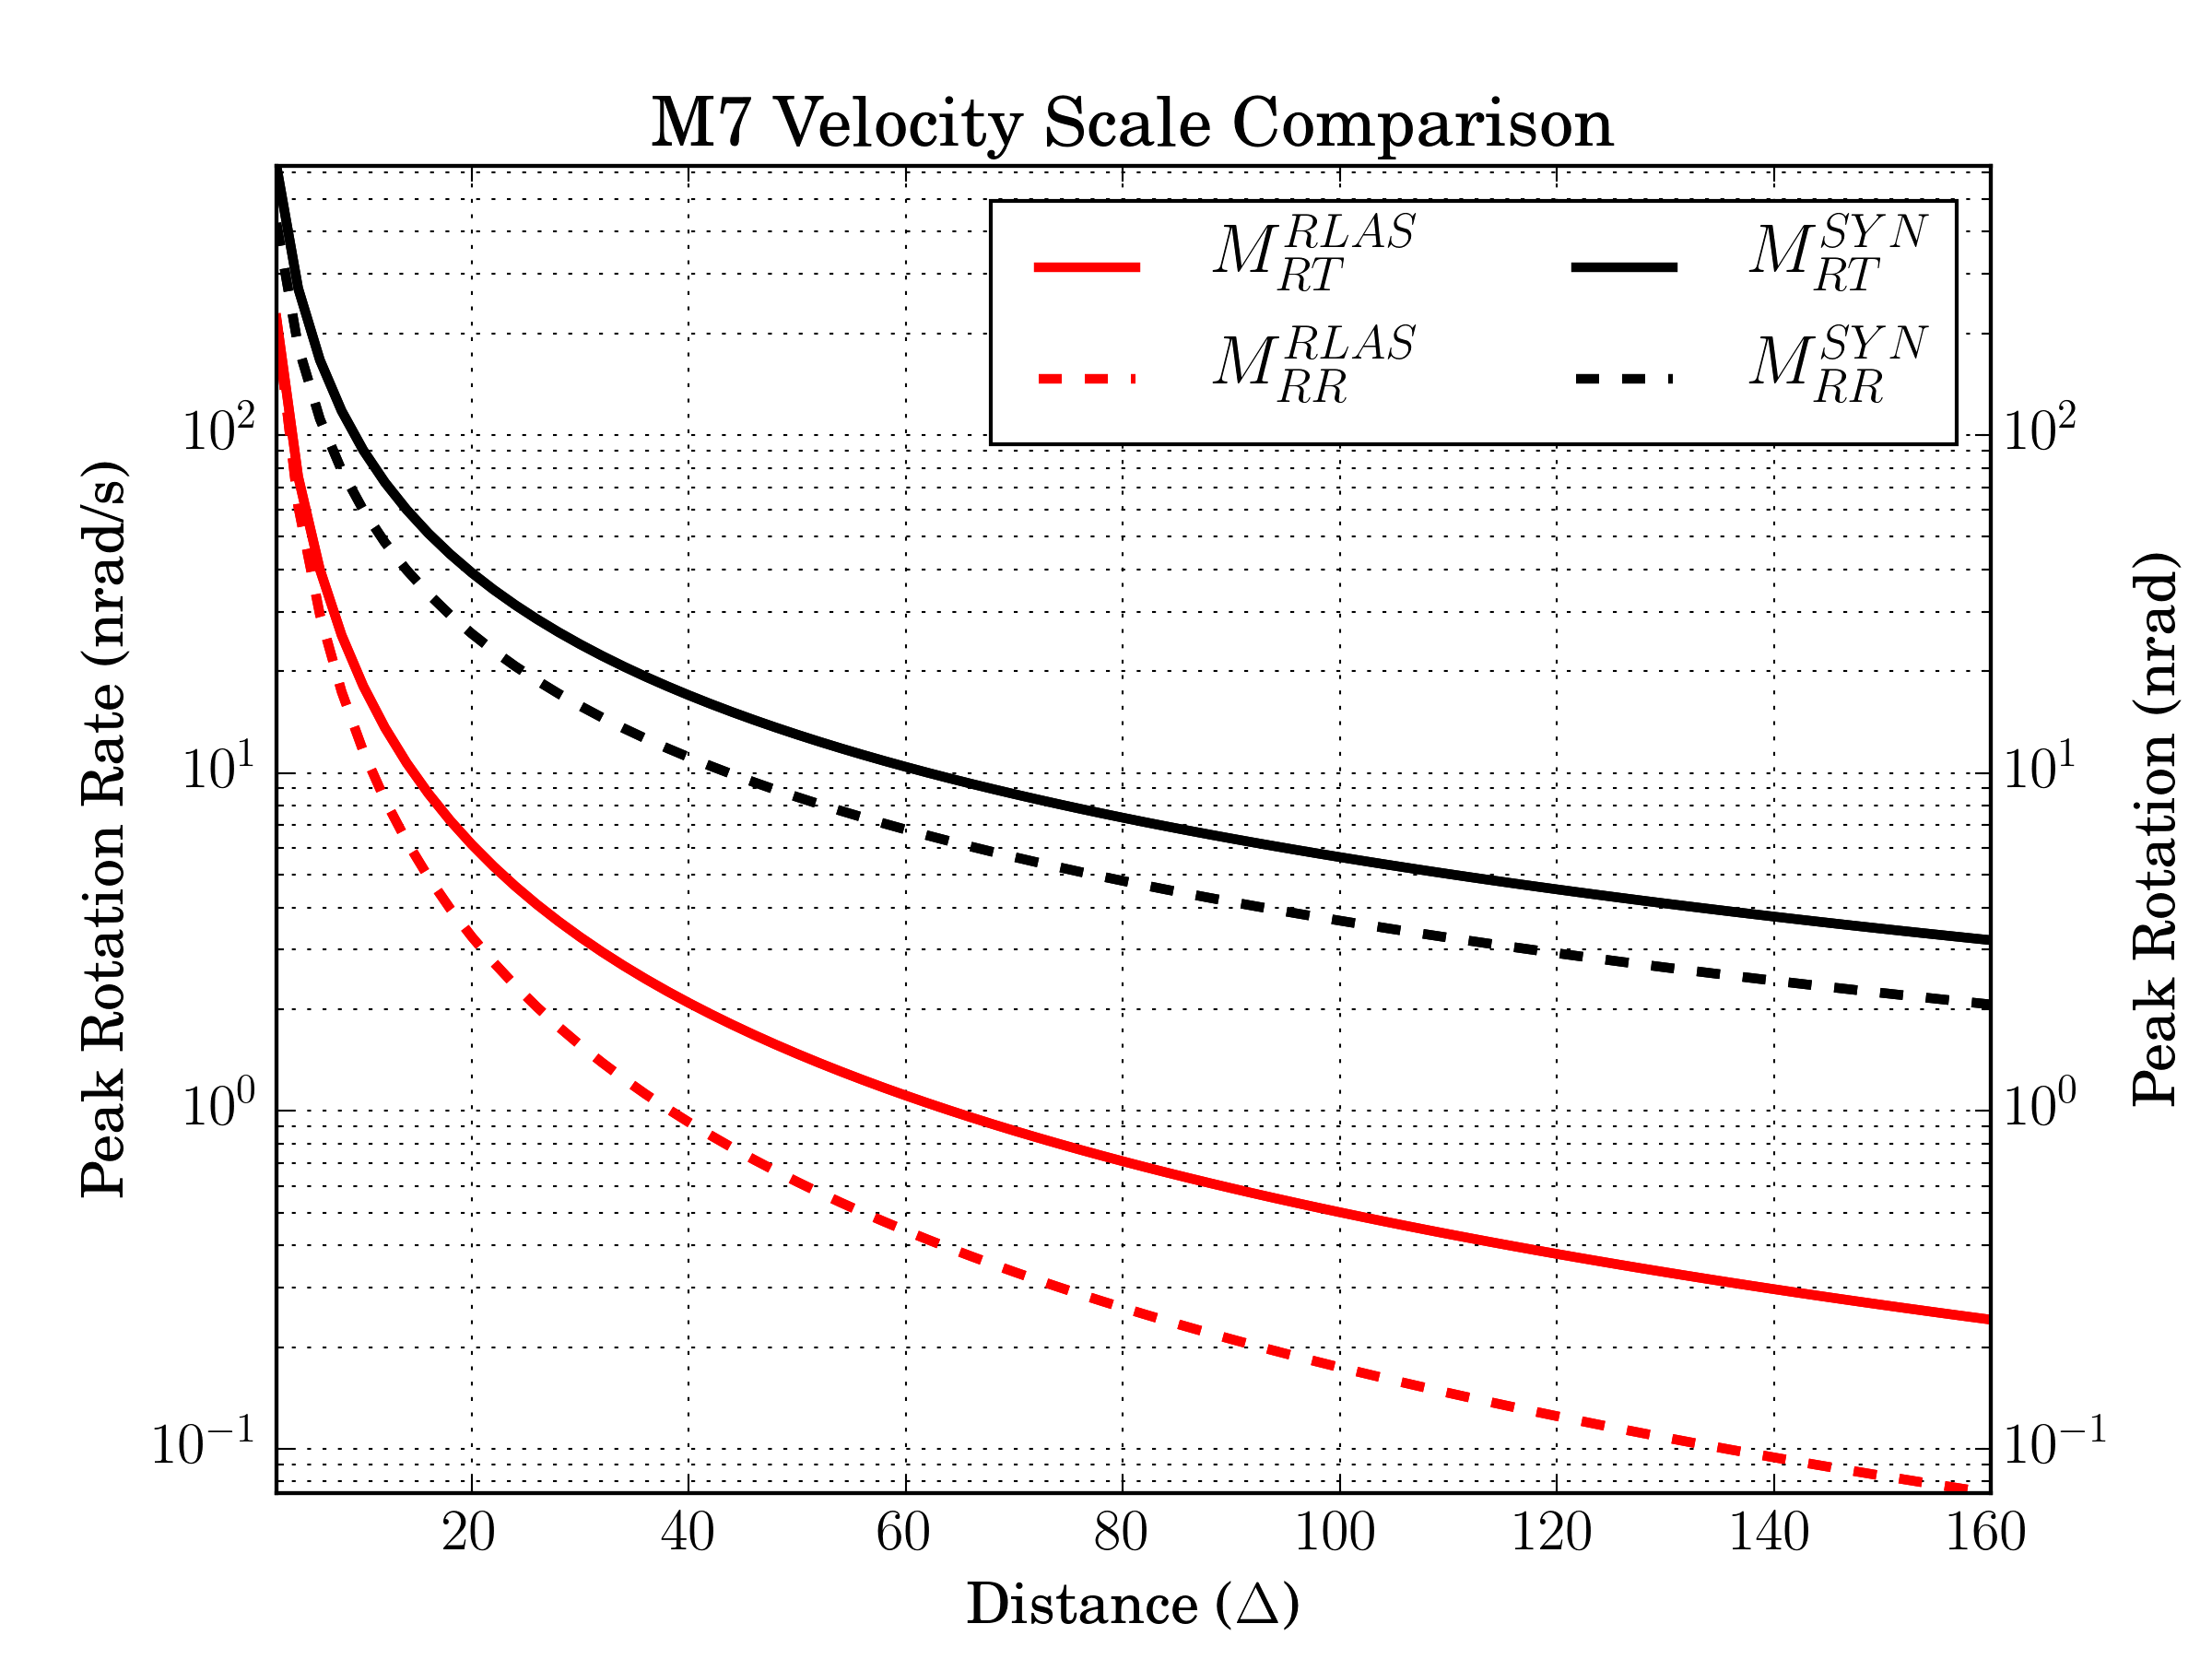
\includegraphics[width=.5\textwidth]{rrscales}}
\caption{A comparison of rotation based scales for station WET and synthetic scales. Peak amplitudes given in units of nanoradians/s [need to change or remove incorrect figure title]}
\label{fig:rr_scale}
\end{figure}

Confidence intervals, which can be viewed as a quantification of misfit between the magnitude equation we fit and the observations, shows the uncertainty of the observations due to the limitation of spatial coverage; in Figure \ref{fig:rr_obs}, the red shaded area shows the confidence interval of the M6 decay line. Relatively large uncertainties arise from the large scatter between predicted and expected amplitudes.% add some explanation on confidence intervals
It should be noted that the magnitude scale is heavily controlled by its end members. Due to a lack of events at very close epicentral distances, it is difficult to constrain the decay here, and the few events at distances less than 20$^\circ$ have a strong influence on the derived value of B. It can also be seen that more than one third of the events used in this study fall around 80$^\circ$ epicentral distance, due to geographic constraints; many of these events occur around Japan, as seen in Figure \ref{fig:event_map}.  

%Discussion: comparing regional view vs an averaging
\subsection{Observed and synthetic waveforms}
Most of the synthetically generated seismograms waveforms were compared with their observation counterparts. In one event (2010-07-18), a fore shock in the observations obscured arrivals and prevented useful comparison. In most cases, P-wave and S-wave arrivals matched well. Later arrivals are not in agreement with very different surface wave behavior. 

%put this into discussion
This can potentially be explained by the use of point sources for such large magnitude earthquakes; the effects of the source time function as well as the rupture plane are not captured in our synthetics, and we therefore do not expect to match phases of surface wave arrivals. Consideration should also be given to the topographic and crustal models included, which affect the resulting surface wave waveforms. The broad frequency range (10-60s) also present difficulties in matching waveforms. Narrow pass filters (i.e. 20 second dominant period) capture similarities better, however we aim to stick to the definition of the IASPEI surface wave magnitude equation, which calls for this broad frequency range. Fortunately in this study, we focus on peak amplitude measurements and therefore are not heavily impacted by the misfit of waveforms.

%traces only extend one hour?

Comparisons of transverse acceleration and rotation rate provide solid phase matching throughout the waveform, with the strongest correlation during the surface wave train, even for relatively wide bandpass filters (i.e. 10 to 60 seconds). This is true for both observations and synthetics.


\subsection{Synthetic magnitude scales}
Results derived from synthetic seismograms, shown in Table \ref{tab:scales}, vary quite dramatically from the observations. Synthetic results do not reflect the same discrepancies that are present in the values given by observations.

A visual representation for the synthetic rotation rate magnitude scale $M_{RR}^{SYN}$ is shown in Figure \ref{fig:syn_scale}. The distribution of points on this scale is much more uniform compared to \ref{fig:rr_obs}. This can be attributed to the substantially larger number of recordings for a single event due to the large number of synthetic stations. With so many station receiver pairs over a range of epicentral distances, there are roughly six times more observation points, which provides stronger coverage of epicentral distances. The number of events at very close distances is also quite low, similarly due to the imposed geographic limitations. The 95\% confidence intervals provide a much narrower band, due to the very consistent spacing of points for a single event; capturing a single event over the entire distance range puts a strong constraint on the fitted decay constants.
%look at equation for confidence interval, what controls it

The synthetic magnitude scales all exhibit very similar values for the decay constant B. The large variation seen in the observations is not captured here. Compared to the IASPEI magnitude scale, all values of B for derived synthetic scales fall lower. Synthetic rotation rate gives the largest, or steepest decay constant at 1.215, but only by a negligible margin. Looking at the values of C, expected amplitudes are all also quite high, except for rotation rate.

\begin{figure*}
\centerline{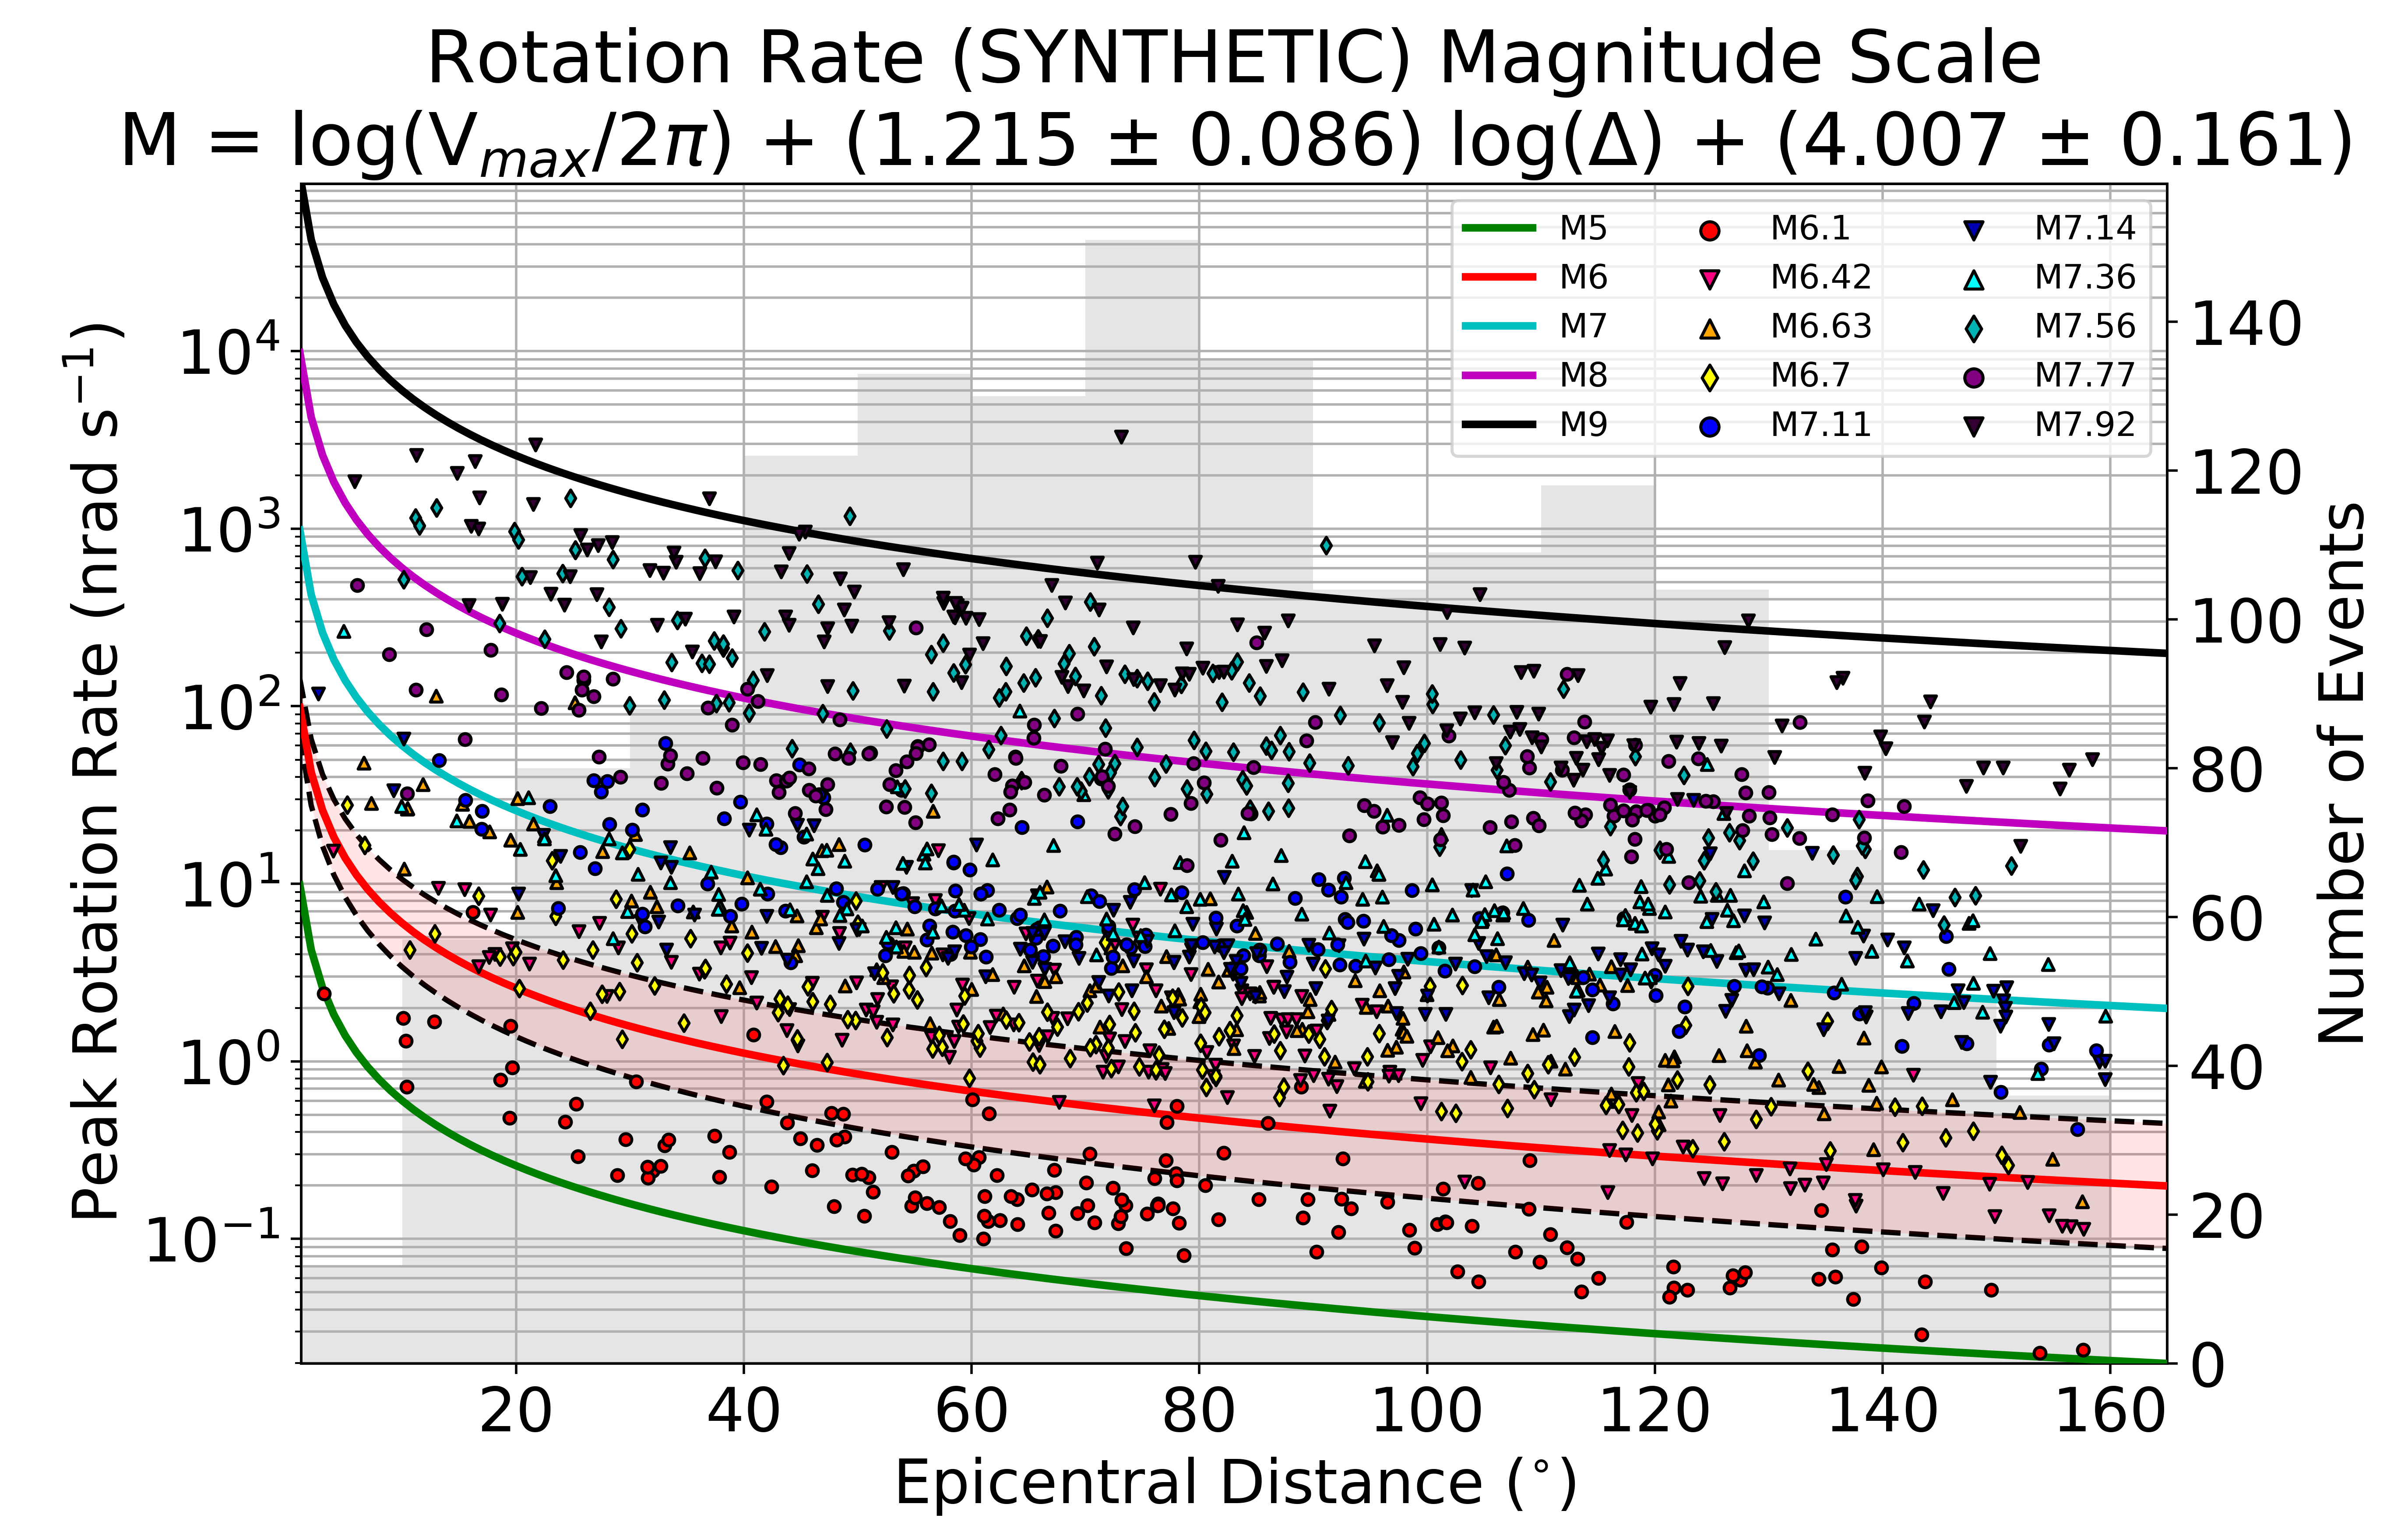
\includegraphics[width=0.8\textwidth]{RR_SYN}}
\caption{Rotation rate magnitude scale for synthetics. All objects similarly represented as in Figure \ref{fig:rr_obs}. Colors of points here represent individual events simulated (for event information, see Table \ref{tab:syn_events}). Scatter from a perfect decay curve potentially due to the effects of varying travel paths through the 3D crustal and mantle models, amplified by the random distribution of source-receiver pairs.}
\label{fig:syn_scale}
\end{figure*}

\begin{table*}
\begin{minipage}{115mm}
	\begin{center}
		\begin{tabular}{ |l|c|c|c|c| } 
		        \bf{Scale} & \bf{Label} & \bf{B} & \bf{C}  & \bf{Wave}\\ \hline
        IASPEI & $M_{S}^{BB}$ & 1.66 & 0.3  & Rayleigh \\ \hline
        Herak Herak 1993 & $M_{S}^{HH}$ & 1.094 & 1.429  & Rayleigh \\ \hline
        Ambraseys-Free 1997 & $M_{S}^{AF}$ & 0.947 & 1.77  & Rayleigh \\ \hline
        Vertical Velocity (Wettzell) & $M^{WET}_Z$ & 1.084 $\pm$ 0.264 & 1.093 $\pm$ 0.511  & Rayleigh \\ \hline
        Vertical Velocity (FFB) & $M^{FUR}_Z$ & 1.095 $\pm$ 0.259 & 1.09 $\pm$ 0.502  & Rayleigh \\ \hline
        Rotation  & $M^{RLAS}_{RT}$ & 1.557 $\pm$ 0.295 & 4.186 $\pm$ 0.569  & Love \\ \hline
        Rotation Rate & $M^{RLAS}_{RR}$ & 1.823 $\pm$ 0.303 & 4.113 $\pm$ 0.586  & Love\\ \hline 
        Transverse Velocity (Wettzell) & $M^{WET}_T$ & 1.45 $\pm$ 0.27 & 0.527 $\pm$ 0.521 & Love \\ \hline
        Transverse Velocity (FFB) & $M^{FUR}_T$ & 1.442 $\pm$ 0.27 & 0.447 $\pm$ 0.523 & Love \\ \hline

		\end{tabular}
		
    		\caption{Magnitude scales and derived constants with 95\% confidence intervals for observations at instruments RLAS, WET (Wettzell, Germany) and FUR (F\"urstenfeldbruck, Germany), for equations of the form $M = log_{10}(V/2\pi) + B\cdot log_{10}(\Delta) + C$. The final column gives consideration to the wave type that each instrument component should provide a proxy for.}
		\label{tab:scales}
	\end{center}
	\end{minipage}
\end{table*}

\begin{table*}
\begin{minipage}{115mm}
	\begin{center}
		\begin{tabular}{ |l|c|c|c|c| } 
		        \bf{Scale} & \bf{Label} & \bf{B} & \bf{C}  & \bf{Wave}\\ \hline
        Synthetic Rotation  & $M^{SYN}_{RT}$ & 1.204 $\pm$ 0.086 & 3.841 $\pm$ 0.159  & Love \\ \hline
	Synthetic Rotation Rate & $M^{SYN}_{RR}$ & 1.215 $\pm$ 0.086 & 4.007 $\pm$ 0.161  & Love\\ \hline 
        Synthetic Transverse Velocity & $M^{SYN}_T$ & 1.094 $\pm$ 0.081 & 0.146 $\pm$ 0.16 & Love \\ \hline
        Synthetic Vertical Velocity  & $M^{SYN}_Z$ & 1.206 $\pm$ 0.08 & -0.011 $\pm$ 0.149  & Rayleigh \\ \hline
		\end{tabular}
		
    		\caption{Same as Table \ref{tab:scales}, but for magnitude scales derived with synthetic seismograms.}
		\label{tab:syn_scales}
	\end{center}
	\end{minipage}
\end{table*}


\subsection{Expected rotation amplitudes}
One useful aspect of magnitude scales is to provide an expected amplitude value for a given magnitude event at certain distance. One area of interest in rotational seismology is the development of field deployable sensors. Due to the low order of magnitude of rotation amplitudes (teleseisms measured in nanoradian scale), it is of concern whether newly developed field deployable rotation sensors can reach the sensitivity necessary to capture the rotational motion amplitudes excited by regional or tele- seismic events. With the rotational magnitude scale derived here, we are able to create a list of observation-based expected amplitudes. At the time of writing, the field deployable rotation sensor BlueSeis from the company iXBlue, has a noise floor of roughly 1 nrad/s/$\sqrt{Hz}$ \cite{bernauer2018blueseis3a}. Referring to Table \ref{tab:scales}, the approximate maximum distance the sensor can be placed to detect a M$_w$5 event would be 21$^\circ$ epicentral distance, roughly 2300 km. This distance range would mean current day sensors could detect regional $>$M5 earthquakes. Other considerations must be taken into account before these values can be used for field deployment decisions, however it provides a useful approximation for future instrument deployments.

%smallest events discernible on observatory based rlas?


\section{Discussion and Conclusions}
% motivation for the work
The long term continuous recordings of rotation and translation waveforms at Wettzell has provided an extensive catalog of colocated observations to explore four components of seismic signals, for events of varying source parameters and travel paths. The motivation for addressing amplitude decays in the initial study of Igel et al. \shortcite{igel2007broad}, was to determine whether or not decay of peak observed rotation rates was consistent with the definition of the commonly used surface wave magnitude equation. In this study we expanded our motivation to include the comparison of decay rates between rotations and translations, to see if, and how, these quantities might differ. Measurements of seismically induced rotation amplitudes have never been addressed on such a scale, and  if rotation measurements should someday be incorporated into standard seismological practices, it is useful and beneficial to understand the general characteristics of their observed signals.

%discussion of results
In this paper we set out to determine whether amplitude decay for observed rotations differed from those of translations. The rotation based magnitude scales in Table \ref{tab:scales} present the idea that rotation amplitude decay is not exceedingly different from those for translation measurements; that is, values of B are not orders of magnitude different. Since rotation measurements in the surface wave train sample the horizontal nature of the Love wave, this finding is not so surprising, and of course was already shown previously by Igel et al. \shortcite{igel2007broad}.

Although translation measurements exhibit varied decay characteristics, it has been previously shown that this result is not unexpected. Corrected values of the coefficients B and C have been proposed using a global catalog \cite{herak1993distance} and a European regional dataset \cite{ambraseys1997surface}. These corrections match well with the vertical velocity scales derived in this work; the values (adjusted for the change of units in the IASPEI scale) are presented in Table \ref{tab:scales} as $M_S^{HH}$ and $M_S^{AF}$ for corrections proposed by Herak \& Herak \shortcite{herak1993distance} and Ambraseys \& Free \shortcite{ambraseys1997surface}, respectively. Table \ref{tab:scales} shows that amplitude decay of rotations, sensitive to Love waves, is larger than those of translations sensitive to Rayleigh waves, which suggests that Love waves have a faster amplitude decay rate  compared with Rayleigh waves; using a single catalog of events and colocated measurements reinforces this point. Taking transverse velocity into consideration, which is effectively sensitive to both horizontal components, also shows how a mixture of Love and Rayleigh wave effects averages the value of amplitude decay.

Synthetic results prove drastically different from those predicted by observations, and warrants the doubt whether our synthetics contain the detail necessary to fully capture the reality of an earth structure which strongly affects amplitudes of surface waves. 3D crust and mantle models, including topography and a host of other factors that play a role in surface wave amplitudes, still predicted amplitudes one order of magnitude larger than those observed at our stations. Considerations should be made for the lack of realistic sources, however order of magnitude discrepancies seem too large to pin on a single problem. This large discrepancy points to a need for a more detailed and realistic full earth model than what is available at this time, if it is to be used for this purpose of determining correct amplitudes.

%questions that arise from the results
It still remains to be seen whether these results will hold for measurements made in other geologic settings and on different measurement methods of rotation (e.g. intertial sensors, or array methods). However this pilot study provides a significant breadth of data as a starting point. A lack of observations at epicentral distances less than 20$^\circ$ and greater than 140$^\circ$ provides large uncertainties, so going forward, it would be immensely beneficial to obtain measurements at these distances to provide further constraint. The inclusion of more stations recording the same event would also make these derived scales much more robust. 

%closing paragraph
Measurements of rotations and spatial gradients has proven a very interesting theoretical aspect of a field which has become extremely proficient in stable observations of three translational components. With this new observable, we are able to revisit theories, proposed decades before, with a new perspective. With the development of translational and rotational magnitude scales, we have determined some stark differences in observed amplitude decays between these two observables, and believe we can put forth the idea that Love waves exhibit stronger observed amplitude decays compared to Rayleigh waves, and that perhaps it is necessary to split our current definition of surface wave magnitude into two definitive definitions. Time will tell whether these results hold, as rotation measurements become more readily available and accessible, however it is exciting to see how these might change as a new slew of instruments and observations become available to the field of seismology. 


%to add: 
%-basin amplification of love vs rayleigh waves, transverse component shows on average higher amplitude
%-synthetic stations
%-high frequency attenutation of rotation rate compared to rotation
%-averaging of earth structure not done here
%-confidence interval
%-because of the logarithmic nature of magnitude scales, even differences in the decay constant don't make that much of an impact on the resulting expected amplitudes that one sees 
%-using the same value of c for all rotation, at 80 degrees you get an order of magnitude difference in expected amplitude for synthetic and observed scales
%-because we use Mw and therefore Ms as a controlling parameter in our linear regression, it has a strong effect on the end result for our fitted line
%-dispersion on the synthetics is not as strong as in the observations, which leads to a 'bunching up' of surface waves and incorrect arrival times based on surface wave speed
%
%misc:
%how to convert from old magnitude scales to new - just subtract 3 from C (rewriting of magnitude equation)
%
%+ considerations for observations and synthetics - geographical, data, frequency wise
%+ observation results by themselves
%+ synthetic results by themselves
%+ comparisons of observations and synthetics
%+ questions that arose from the processing
%+ further work

\bibliographystyle{apalike}
\bibliography{biblio.bib}

\label{lastpage}


\end{document}


%\begin{figure}[h]
%\centerline{\includegraphics[width=0.8\textwidth]{XYZ}}
%\caption{XYZ}
%\end{figure}
